\section{Introduction}
\subsection{Background and Motivation}
Analgesics play a vital role in acute and chronic pain management and are among the most consumed and widely available classes of drugs globally \cite{Jaeschke2015}. The ubiquitous presence of non-steroidal anti-inflammatory drugs (NSAIDs) such as Ibuprofen, and other common analgesics like Paracetamol, is a core component of modern healthcare. Despite their widespread use, however, many have adverse side effects that can be more serious than suspected, ranging from mild discomfort to life-threatening outcomes and sometimes death \cite{Harirforoosh2013}. 

While a vast amount of data exists to assess these risks, much of it is critically fragmented. The FDA's (U.S. Food and Drug Administration) Adverse Event Reporting System (FAERS) contains millions of real-world patient reports, but this information has an inconsistent structure and cannot be integrated directly \cite{FDA2023faers}. As a result, performing a clear, comparative analysis of drug safety profiles is challenging, particularly when it comes to fatal outcomes. This challenge of integrating heterogeneous data from various sources is a well-known problem within health informatics \cite{Häyrinen2014}.
\subsection{Problem Statement}
The main problem that was encountered is the following: data in many places. We have data in openFDA we have data in other places, but unifying them is what makes the whole analysis difficult. The fundamental challenge this thesis confronts is the fragmentation of pharmacovigilance data. Important information regarding adverse events, patient demographics as well as regulatory status, resides in disconnected storage spaces. 

The stakeholders which in this case are clinicians, regulatory bodies and legal experts are unable to answer critical and integrated questions, such as: “Is the real-world risk profile of common OTC (over-the-counter) drugs comparable to that of drugs which are barred behind a prescription, based on how often severe and or fatal outcomes occur?” Here we have identified a clear gap and need for an integrated and queryable model at the intersection of pharmacovigilance and regulatory compliance.

In essence, the core problem is a missing semantic model designed to specifically compare the most severe risks, especially those fatal events of the most common painkillers relative to their legal status. This thesis proposes the solution: a structured framework to make the data interoperable, queryable and transparent.
\subsection{Key Terms and Definitions}
Before we dive into the methodology, this section aims to provide definitions for the core technologies and concepts that were central for the underlying thesis. 
\subsubsection{Ontology}
An ontology is a core component of Semantic Web technologies. Its purpose is to serve as a formal and machine-readable model of a specific domain. As a result a widely accepted definition would describe an ontology as a “a formal explicit description of concepts in a domain of discourse” \cite{Noy2001}.

Practically meaning that its purpose is to act as a foundational scheme or “blueprint” for a knowledge graph. This can be achieved by defining the key concepts as well as the rules that are supposed to govern them. This would involve the definition of primary classes of things that exist within the pharmacovigilance domain, such as "Drug", "Patient", and "AdverseEventReport". Likewise the inclusion of data properties, which describe the attributes of each class, for example that a "Patient" has a "patientAge" property and the definition of object properties, which would make sure that the relationships between these classes exist (e.g. "Patient" experiences a "SideEffect"). As a result one will end up with an ontology that ensures that both humans and computers have a shared understanding of the information.
\subsubsection{Knowledge Graph}
When it comes to knowledge graphs, they are defined as “a set of interconnected typed entities and their attributes,” \cite{Pan2017exploiting}. Meaning that the ontology defines the vocabulary of the graph. In this thesis the knowledge graph developed here, represents painkillers, adverse event reports, patients as nodes and the relationships between them as edges. Each edge is a defined connection that links two nodes together, which leads to a simple “subject-predicate-object” statement, also known as a triple. Thus through the connection of thousands of those triples, the source data gets transformed into a queryable network. Ultimately enabling a level of querying that a traditional database could not allow. 
\subsubsection{SPARQL}
This is the standard query language and also the protocol for the Resource Description Framework (RDF), as defined by the World Wide Web Consortium (W3C) \cite{W3C2013sparql}. In general SPARQL is to a knowledge graph what SQL is to a relational database. This thesis makes use of the language to ask analytical questions of the final created knowledge graph. SPARQL goes beyond simple data retrieval, since it lets us construct complex queries that can traverse the relationships between different entities within the graph. For instance, one query can start at the “Drug” class, then navigate through the associated “AdverseEventReport” to find the Patient, and then finish the query off by aggregating the findings for all said patients to calculate a result (e.g. their average age). 
\subsubsection{Pharmacovigilance}
This term is defined by the World Health Organization (WHO) as the “the science and activities relating to the detection, assessment, understanding and prevention of adverse effects or any other possible drug-related
problems.” \cite{WHO2002pharmacovigilance}.

At its core, it addresses a fundamentally challenging aspect in medicine. While pre-market clinical trials are of utmost importance to establish the safety of a drug, they are usually conducted on small control groups. Thus concluding that most safety findings become clear after the drug has been used by millions of people in the real world. Therefore pharmacovigilance is the continuous effort to surveillance and monitor real-world effects of post-market drugs. In consequence, this thesis will aim to build a tool for pharmacovigilance. Hereby the goal is to enable a more efficient analysis of the real-world patient reports, to potentially identify new risk signals.
\subsection{Research Questions}
The primary goal of this thesis is to do a design science project involving the creation of a domain ontology. Thus as a guide, the work is structured by the following research questions, which encompass the core stages of the design, implementation and evaluation:
\begin{itemize}
    \item RQ1: Of the selected painkiller drugs, which are the ones associated with the most total, serious and fatal adverse events within the openFDA FAERS database?
    \item RQ2: How is an ontology that should formally represent common analgesics with their U.S. regulatory status and the adverse event data, which was extracted from the openFDA API, following established ontology development methodologies, designed and populated?
    \item RQ3: How can the resulting knowledge graph be queried, analyzing and comparing the risk profiles of OTC vs. prescription painkillers, in order to examine the alignment between regulatory classification and real statistical data?
\end{itemize}
\subsection{Thesis Structure}
The thesis structure is organized as follows to reach the primary goal:
\begin{itemize}
    \item Chapter 2 reviews the theoretical background and related works in pharmacovigilance, regulatory data, and the use of ontologies in biomedicine.
    \item Chapter 3 outlines the methodology, detailing the data collection from the openFDA API, the preparation of the data, and the design of the ontology.
    \item Chapter 4 evaluates the functional capabilities of the populated knowledge graph, presenting the key findings from the analytical SPARQL queries.
    \item Chapter 5 provides a comprehensive discussion and conclusion. It answers the research questions, reflects on key insights and legal implications, discusses the study's limitations, and concludes with a summary of the thesis's contributions and an outlook on future research. 
\end{itemize}
\section{Theoretical Background and Related Work}
This chapter provides the theoretical foundation for the thesis within the existing research landscape. It begins by discussing the specific domain of pharmacovigilance as well as the challenges associated with its data sources, such as the openFDA API. A detailed review of the related work in the field of biomedical ontologies will be provided, where existing resources are analyzed to identify the specific research gap this thesis addresses.
\subsection{Pharmacovigilance and the openFDA API}
As mentioned in the introduction, pharmacovigilance is the science and activities relating to the detection, assessment, understanding, and prevention of adverse effects or any other drug-related problem after they have been released to the market. A primary tool for post-market surveillance is the collection of adverse event reports. The U.S. Food and Drug Administration (FDA) maintains one of the largest such databases, the FDA Adverse Event Reporting System (FAERS), which contains millions of patient-reported outcomes. 

For this thesis, the primary data source is the openFDA API, a publicly accessible platform that provides programmatic access to the FAERS database. This API allows for the retrieval of data related to adverse events, including patient demographics, the drugs involved, the specific reactions (side effects), and the seriousness of the outcomes, such as hospitalization or death. However, as noted in the initial project proposal, this data is often unstructured and inconsistently formatted, with known challenges such as nested JSON structures and inconsistent data entries. Drug names can vary or be misspelled, and the reports themselves are complex nested structures. This lack of a consistent, unified model makes it difficult to query the data semantically across multiple substances and side effects, thereby justifying the need for an ontology to structure and normalize this information for analysis.
\subsection{Related Work in Biomedical Ontologies}
In order to establish a foundation for this thesis, by positioning it within the current research landscape, a review of existing biomedical ontologies was conducted.  The application of Semantic Web technologies, especially when looking at ontologies and knowledge graphs, to healthcare domains, have been especially active as further means to research for over a decade. Demonstrations of researches have shown that there is a value for technologies, that mean to transform tasks for data integration, clinical decision support as well as new drug discoveries \cite{Daconta2003semanticWeb}.When it comes to biomedical ontologies several valuable examples exist, nevertheless each presents some limitations to our specific goals in the thesis, namely the integrated analysis of real-world side effect frequency, as well as patient demographics and lastly the regulatory status. 
\subsubsection*{SIDER (Side Effect Resource)}
One of the more well known resources in this domain is called SIDER (Side Effect Resource). It links thousands of drugs to their known side effects, while also including frequency data, which are directly extracted from the drug labels. However, when it comes to their most significant limitation, the database is no longer actively maintained \cite{EMBLsiderWebsite}. The last update was in 2015, which concludes that the data lacks the last decade of reporting and is therefore unsuitable for a contemporary analysis of pharmacovigilance trends. Furthermore, while it does provide frequency data, it does not contain demographic data about the patients themselves. Thus excluding itself from this thesis.
\subsubsection*{Formal Ontologies: OAE and DRON}
There are other formal ontologies, such as the Ontology of Adverse Events (OAE) and the Drug Ontology (DRON). The OAE provides a deep classification of different types of adverse events, from the molecular to the population level. Additionally the OAE is essential for standardizing the terminology of adverse events \cite{HeGroupOntobee}. Similarly, DRON provides a comprehensive model of the drug's products, including their ingredients and also their roles \cite{OBOFoundryDRON}.

However on the flip side, they are high-level reference ontologies. Meaning that they are not designed to be populated with instance data from individual patient reports. Therefore they do not include the specific data points, which are required here for this thesis, such as side effect frequency, patient demographics and also the regulatory status. Their strong suit lies in ensuring terminological consistency, but this focus on abstract classification makes them inapplicable for the type of analysis performed here. 
\subsubsection*{Proprietary and Restricted Resources: MedDRA and DrugBank}
While comprehensive terminologies that do cover all the necessary concerts exist, they are usually not fully open and accessible. MedDRA (Medical Dictionary for Regulatory Activities) is the industry standard for reporting adverse events. It is remarkable with its rich and hierarchical terminology and is of use for many regulatory bodies worldwide \cite{MedDRA2025}. However, the primary limitation is a commercial license, which disqualifies it for this open-source academic thesis.

DrugBank would be another candidate as a comprehensive resource that would include detailed information, of which the approval status and side effects would get listed up. On the other hand, while it is accessible to academic researchers, its full, machine-readable dataset is restricted \cite{DrugBankWebsite}. To further close off this matter, it does not provide direct access to the real-world patient reports which are the focus in this case. 
\subsection{Methodologies for Analyzing the openFDA Dataset }
To further contextualize this thesis, an analysis of other research projects that similarly utilized the openFDA dataset was conducted. Through this knowledge we can compare our ontological approach to other analytical methods. Much of the existing research of the openFDA data used statistical or even machine learning methods. 

For example, one of the research focuses on creating tools for statistical disproportionality analysis. The OpenVigil FDA project is one of them \cite{Bohm2016openvigil}. Particularly, a  web-based tool is provided, where queries of the openFDA are used to calculate measures like the Reporting Odds Ratio, the Proportional Reporting Ratio and the Chi-squeared value.Thus being useful when identifying if a specific drug and adverse event occur more frequently, then expected by chance. That way, physicians and pharmacists could perform these calculations easily for their clinical questions, in order for the comparison of safety profiles of two drugs for a specific side effect.While this tool is invaluable for traditional statistical detection, it fundamentally differs itself from the work in this thesis. The output of the OpenVigil tool is not a queryable map of the knowledge domain itself. To be more specific, their purpose is to answer “how often” a signal would appear, than to answer questions such as “what”, “why” and “how”, which is the aim here for this context. 

More recently, new projects have been initiated, where graph-based and semantic approaches have been used on the FAERS data. One of such projects is the GRAPH-AID. Here, the key functionality lies in creating a semi-automated workflow for creating an OWL ontology from the FAERS data. This happens after loading it into a Neo4j graph database at first \cite{li2024neuralcorrelateslogicalmathematicalsymbol}. This approach shares a similar goal with this thesis, but its methodological focus differs itself fundamentally. There is a key difference though: the work of this thesis is not focused on the automated generation of a schema, but rather on the manual design of a specific model that is purpose built for multi-dimensional risk analysis. The GRAPH-AID project however emphasizes the development of a user-friendly pipeline to help other users who are not as experienced in the description and generation of an ontology. The final analytical capabilities of the then resulting model are not their primary focus. 
\subsection{Comparison of Related Work}

\begin{table}[htbp]
\centering
\small
\begin{tabular}{|p{1.7cm}|p{2.0cm}|p{3.6cm}|p{1.7cm}|p{2.4cm}|}
\hline
\textbf{Tool} & \textbf{Access} & \textbf{Data Scope} & \textbf{Status} & \textbf{Focus / Format} \\
\hline
SIDER & Public & Side Effects \& Frequency (Not Integrated) & Outdated (2015) & Data Curation (CSV/RDF) \\
\hline
OAE / DRON & Public & Terminology Only (Not Integrated) & Updated & Terminology (OWL) \\
\hline
MedDRA & Commercial & Side Effects \& Terminology (Integrated) & Updated & Terminology (Proprietary) \\
\hline
DrugBank & Partial & Approval Status \& Side Effects (Integrated) & Updated & Data Curation (CSV/API) \\
\hline
openFDA & Public & Patient Reports \& Side Effects (Requires Integration) & Updated & Raw Data (JSON) \\
\hline
\textbf{This Thesis} & \textbf{Open Source} & \textbf{All-in-One: Patient Reports, Side Effects, Demographics (Integrated)} & \textbf{Current} & \textbf{Integrated Analysis (RDF)} \\
\hline
\end{tabular}
\caption{Comparison of Related Work.}
\label{tab:related_work_comparison}
\end{table}

As the Table \ref{tab:related_work_comparison} illustrates, while the openFDA API serves as the foundational data source for this project, it is best understood as a provider of raw material. Meaning that the API alone does not offer an integrated view of regulatory status. The contribution of “This Thesis” is the creation of a new system, which means to integrate the data from the API endpoints into a structured ontology. The data knowledge graph will be queryable and used as an analytical tool.
This review of related work reveals that there is a specific gap. While many valuable resources exist, they seem to operate in silos: formal ontologies provide the rules but lack the real-world data.Curated databases provide clean data, but suffer from the absence of raw patient reports. Public APIs provide the reports, but miss a formal queryable structure. This review concludes that there is no single, up-to-date and openly accessible ontology that integrates drug approval status with detailed real-world adverse event data. Of which the patient demographics and side effect frequency is included, by populating the ontology from a public API. 

Thus the thesis directly tries to address the gap by creating a new focused ontology populated with current data from openFDA, providing a resource, so that comparative risk analysis of common painkillers can be enabled. It is not about creating another ontology, another database or another data script. It is about creating an integrated system. 
\section{Methodology}
This chapter details the systematic approach that was taken to address the research gap identified in the previous chapter. A design science research paradigm serves as the foundation for the methodology, which is an appropriate choice for the creation and evaluation of a technical artifact like the proposed ontology. The process was guided by the LOT (Linked Open Terms) methodology, as it provides a structured and iterative base for ontology building.

The following sections will outline the key stages of this project: the data collection and preparation, the subsequent ontology design and validation, and the final implementation and population of the knowledge graph.
\subsection{Data Collection and Preparation}
Data is the foundation of any ontology. A programmatic approach was taken to extract the data from the openFDA drug/event API. This method was chosen over a manual download of datasets, so that the data collection process could be transparent and repeatable as well as adjustable. 

The python script developed for this thesis integrates several libraries and a public API. The implementation was guided by best practices as well as official documentation for these core components. The request library is known as the standard for making HTTP requests in python. All of the API calls to the openFDA were made with the use of this library, where the methods were followed in the official documentation \cite{requestsDocumentationHHTPForHumans}. When it comes to the pandas library, the tool is utilized for manipulation in python. Here it was used for the structuring of the nested Json data returned by the API, so it could produce clean tabular CSV files \cite{pandasDocumentation}. Finally all the queries were constructed according to the official documentation for the openFDA API. In consequence specifying how the correct endpoints are supposed to look in order to query parameters like search and count, and ultimately the structure of the returned data \cite{openFDA_API}. To ensure that all the dependencies were localized, the script was initiated within a venv (virtual environments).

It is important to note that for the purpose of this thesis, only a sample of the data was collected. The aim was not to perform a study of all million reports, but rather to collect a dataset that would be sufficient in size to validate the functionality of the knowledge graph.  That way, we can focus on the methodological contribution of creating a tool that could later be scaled up to the full dataset. 

The script was designed so that the output would result in two CSV files that serve as the base for the knowledge graph, so that all of the projects research questions could get addressed:

\begin{enumerate}
    \item \textbf{Aggregated Statistics and Regulatory Data (\href{https://github.com/zerdapt/bachelor-thesis/blob/main/data/raw/drug_risk_summary.csv}{\nolinkurl{drug_risk_summary.csv}}):} This is a high-level summary for each common painkiller. The data points are: name, U.S. regulatory status (“OTC”, “Not Approved in US”) and aggregated counts for total, serious and fatal adverse event reports. This file is needed to answer RQ1 directly, and also serves as a basis for calculating the fatal report percentages in the later stages of this thesis.
    \item \textbf{Individual Report Details (\href{https://github.com/zerdapt/bachelor-thesis/blob/main/data/raw/fatal_report_details.csv}{\nolinkurl{fatal_report_details.csv}}):} This file represents the more specific details from the individual patient adverse event reports. For each drug a sample of reports was requested from the API. Specific granularities such as the reported side effects (MedDRA terms), patient age, sex and the country of origin of the report were extracted. Furthermore each record has a unique identifier for the analgesic involved, enabling a cross-link between the two sets of data.This is especially needed to answer the RQ3.
\end{enumerate}
This data collection strategy was chosen to enable a sophisticated statistical analysis, so a deep investigation could be achieved for the final knowledge graph. The following section will detail the specific implementations within the python script, to show how the two csv files were generated. However, the complete source code will be available in the project's GitHUb repository under /src. 
\subsubsection{Script for Aggregated Data Collection}
The first part of the script had its focus on the generation of the \texttt{drug\_risk\_summary.csv}. To establish that the code was clean and maintainable. The key configuration variables were defined at the beginning of the script, such as the base URLs for the API endpoints. 

\begin{lstlisting}[language=Python, caption={API base URLs defined in the script.}, label={lst:api_urls}, captionpos=b]
EVENT_BASE_URL = "https://api.fda.gov/drug/event.json"
LABEL_BASE_URL = "https://api.fda.gov/drug/label.json"
\end{lstlisting}

In order to achieve the goal, the script had to perform two key tasks for the painkiller. One of which was to determine the US regulatory status and the other was to fetch the aggregated report counts. 

For the first part, the obtaining was reached by querying the drug/label endpoints. In order to ensure robustness the use of a synonym dictionary (\texttt{DRUG\_SYNONYM}) was implemented. For instance, for the purpose of searching the status of paracetamol, the script will search for both “PARACETAMOL” but also its US market name “ACETAMINOPHEN”. Then, in order to find the regulatory status, it will extract the \texttt{product\_type} from the API response and classify the drug as “Over-the-Counter”, “Prescription” or “Not Approved in US” if the label is not found. 

Now, to get the total, serious, and fatal report counts, the script makes a series of targeted calls to the \texttt{drug/event} endpoint. Instead of using the \texttt{count} parameter, it leverages an efficient feature of the API: by setting the \texttt{limit} parameter to \texttt{0} in a \texttt{search} query (e.g., \texttt{search=...\&limit=0}), the API returns only metadata, including the total number of matching records. This method avoids downloading large datasets and provides the exact counts needed to answer RQ1.
\subsubsection{Script for Detailed Fatal Reports}
The second script is slightly more complex and created a sample of individual fatal reports for the \nolinkurl{fatal_report_details.csv} file. To control the scope together with the quality of the sample, the following parameters were defined at the top of the script:

\begin{lstlisting}[language=Python, caption={Key parameters for fatal report sampling.}, label={lst:fatal_params}, captionpos=b]
FATAL_EXAMPLES_TO_FIND = 10
IDS_TO_CHECK = 50
AGE_UPPER_BOUND = 140
\end{lstlisting}

The steps of the creation consisted of the following:
\begin{enumerate}
    \item First the script had to query the API to find a list of \nolinkurl{safetyreportids} for reports that are marked with the value of \nolinkurl{seriousnessdeath} being 1. Meaning we had to look for all the reports where the patient passed on.
    \item Then we had to minimize the confounding variables, so that the script filters the list of potential IDS to include only the reports where the painkiller in question was the only suspect drug listed for the side effects. Otherwise it would be hard to pinpoint, which drug really was at fault for the outcome. That way, the clarity of the sample data would be ensured.
    \item For the remainder of the report IDs the script then had to find their full report data. But before doing so it had to check whether or not the report contained all the necessary data points for the analysis, such as valid patient age, patient sex, and the country where the report occurred. If the report did not include all of the above, then the report id was discarded.
    \item Only after a report has been both filtered and validated, its data could finally be extracted into the \nolinkurl{fatal_report_details.csv} file.
\end{enumerate}
The steps had to be rigorous, to ensure that the final knowledge graph could actually get populated with a well structured and complete dataset, so we could proceed with the semantic analysis in the following chapters. 
\subsection{Ontology Design and Validation}
To design and implement the ontology, required a structured process. The primary tools used for this was Protégé, which is an open-source ontology editor, providing the environment for creating and managing the classes, properties as well as relationships. For the data preparation, Ontotext Refine was instrumental in the cleaning of the raw CSV data from openFDA. In addition to that, Ontotext Refine allowed the transformation of the cleaned data into the structured Resource Description Framework (RDF) format, which is essential for the population of the ontology. 
\subsubsection{Ontology Design and Implementation}
The initial design was straightforward and centered on a \texttt{Drug} class and a \texttt{Report} class. However, in the early modeling, a challenge began to arise: when attaching patient details such as \texttt{patientAge} directly into a Report, created a ``flat'' model. Thus limiting the analytical possibilities. It would not have been possible, for example, to ask questions about the patients themselves.

To solve this problem, the model was reworked into a more interconnected structure. This revised approach ensures that each entity is represented by its own class, allowing a more accurate representation of the domain.Thus the final ontology is built around the following set of classes:
\begin{itemize}
    \item \textbf{\texttt{Drug}}: Represents the painkiller medications. Each drug individual (e.g. Ibuprofen) acts as an anchor for its properties such as \texttt{totalReportCount} and \texttt{fatalReportCount}.
    \item \textbf{\texttt{AdverseEventReport}}: This class represents a single adverse event report from the openFDA dataset. Each instance of this class is linked to the specific \texttt{Drug} and the \texttt{Patient} it involves.
    \item \textbf{\texttt{Patient}}: Represents the individual person who experienced the side effect, enabling a detailed demographic analysis.
    \item \textbf{\texttt{SideEffect}}: This class models the side effects as their own classes, rather than simple text strings, which allows for a comparative analysis across different drugs.
    \item \textbf{\texttt{RegulatoryStatus}}: Here the legal US status of a drug gets modeled as a class.
    \item \textbf{\texttt{Region}}: Represents a geographical location, which is primarily used to specify the county where the adverse event report originated.
\end{itemize}

The implementation of the model was initiated in Protégé with the use of the Web Ontology Language (OWL). This involved the process of defining the schema, establishing all relationships and making sure that there is a logical consistency of the model.
The ontology was annotated with the essential metadata using Dublin Core (DC) term to ensure a proper attribution. This involved the ontologies \texttt{terms:title}, \texttt{terms:creator} and a \texttt{terms:description}. Additionally the \texttt{terms:license} was added, so that the Creative Commons Attribution 4.0 International license could be added. Without that, it would not correctly make the ontology openly accessible as well as reusable.

Classes are connected through a set of object properties that are described by data properties. In order to enhance the logic of the ontology, special characteristics were added to these properties. One of which was defining key relationships with inverse properties to allow bidirectional querying. For example the \texttt{drugHasRegulatoryStatus} property is the inverse of is \texttt{isStatusOfDrug}. Meaning that whenever stating that the drug has a certain status, the reasoner would automatically infer that the status is one of that drug. Another declaration added to the properties was the functional one, for example \texttt{reportConcernsDrug} and \texttt{reportInvolvesPatient}. Concluding that an adverse event report can only concern one drug and one patient at a time. That way inconsistencies can be prevented within the data. Furthermore properties like \texttt{patientExperiencedSideEffect} were declared as asymmetric, conveying that if a patient were to experience a side effect, the side effect would not experience the patient. In addition, it was also assigned as irreflexive, that an individual cannot have this relationship with itself.

Every class, object property and data property in the ontology was also annotated with a \texttt{rdfs:label} as well as a \texttt{rdfs:comment}, to ensure that it is human-readable. That way the ontology can be maintainable for both developers and also domain experts.

The most important of these properties are summarized in Table \ref{tab:ontology_properties}.

\begin{table}[htbp]
\centering
\small
\begin{tabular}{|p{2.6cm}|p{1.8cm}|p{1.8cm}|p{1.8cm}|p{3.0cm}|}
\hline
\textbf{Property Name} & \textbf{Type} & \textbf{Domain} & \textbf{Range} & \textbf{Description} \\
\hline
report\-Concerns\-Drug & Object Property & Adverse\-Event\-Report & Drug & Links a report to the drug it is about. \\
\hline
report\-Involves\-Patient & Object Property & Adverse\-Event\-Report & Patient & Links a report to the patient it involves. \\
\hline
patient\-Experienced\-Side\-Effect & Object Property & Patient & Side\-Effect & Links a patient to the side effect they experienced. \\
\hline
drug\-Has\-Regulatory\-Status & Object Property & Drug & Regulatory\-Status & Links a drug to its legal status. \\
\hline
patientAge & Data Property & Patient & xsd:integer & The age of the patient. \\
\hline
report\-Country\-Code & Data Property & Adverse\-Event\-Report & xsd:string & The country where the report originated. \\
\hline
\end{tabular}
\caption{Summary of key properties in the painkiller ontology.}
\label{tab:ontology_properties}
\end{table}

One of the critical phases includes the ontology validation, to ensure that the ontology is suitable for its purpose. This process not only verifies that the model is structurally sound but it also makes sure that it is functionally capable to meet the requirements within the competency questions. For this thesis, a tree stepped approach was adopted for the validation. First through using a reasoner, second by testing the quality by using the \texttt{OOPS!} tool and lastly by testing if the competency questions can be answered with SPARQL queries, after the ontology has been populated.
\subsubsection*{Technical Validation}
The first step was to ensure that the ontology contained no internal contradictions. This was achieved by using the built-in reasoner in Protégé (e.g. \texttt{HermiT}). This reasoner immediately checks for consistency issues, by inferring new knowledge from the explicitly stated definitions. After executing the reasoner on the entire ontology, the validation process confirmed that the ontology is consistent and coherent. There are no unsatisfiable classes nor logical contradictions.

\subsubsection*{Quality Evaluation: Pitfall Detection}
While the reasoner confirms if the ontology is logically consistent, it does not guarantee that it is designed well. A schema can be free of contradictions but it can still contain structural flaws. The issues, also known as pitfalls, can thus lead to incorrect inferences, which can make the ontology difficult to maintain and reuse in the future.


Therefore, before populating the ontology,  the initial schema  \nolinkurl{ontology_painkiller.rdf} underwent a formal validation process to identify and correct potential flaws. This allows for a functioning structure to proceed with the use of the ontology. The evaluation was done using the Online Ontology Pitfall Scanner (\texttt{OOPS}!). This service tool is widely recognized and  automatically looks for common structural errors, followed by a clear instruction for improvement \cite{oopsWebsite}.

The validation process was initiated by uploading the ontology raw \texttt{RDF/XML} file directly into the scanner’s input field. Thus returning one critical pitfall ``\texttt{Missing disjointness}'' shown in Figure~\ref{fig:oops_pitfall}.

\begin{figure}[H]
\centering
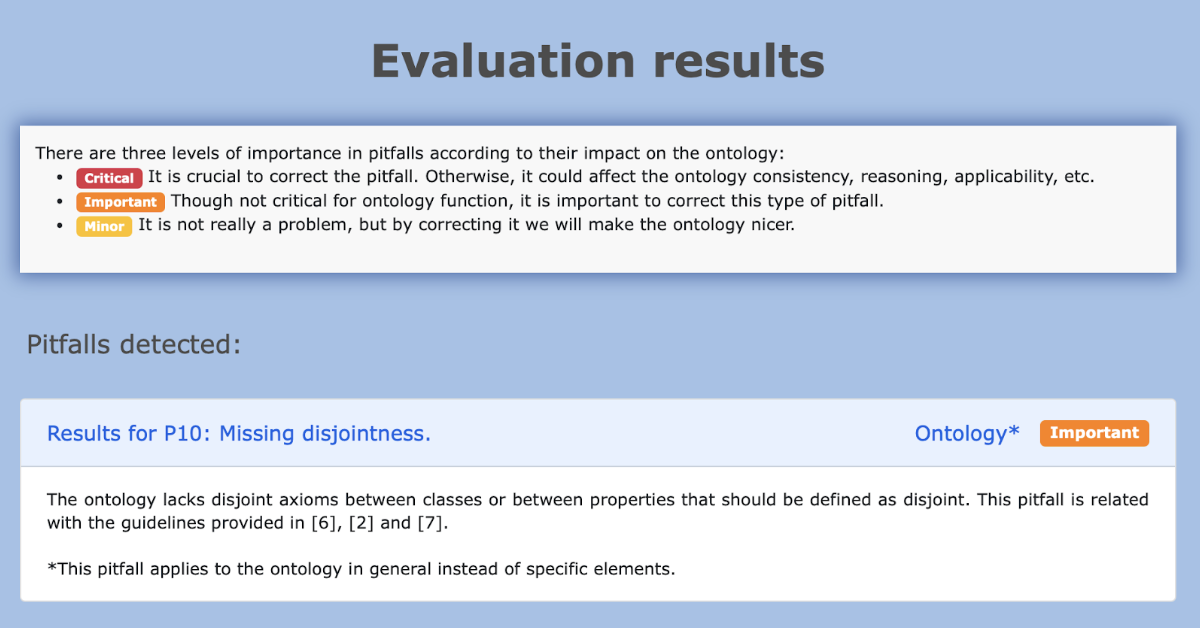
\includegraphics[width=0.9\textwidth]{pitfall_results.png} % Replace with the path to your image
\caption{The OOPS! tool identifying the "Missing disjointness" pitfall.}
\label{fig:oops_pitfall}
\end{figure}

\subsubsection*{Pitfall: Missing Disjointness Between Classes}
The scanner reported that the main classes (e.g. \texttt{Drug}, \texttt{Patient}, \texttt{SideEffect}) were not correctly declared as being disjoint from each other. Without \texttt{owl:disjointWith} axioms, the reasoner cannot conclude that an individual cannot be a member of multiple classes at the same time. Thus potentially leading to wrongful inferences. If we were to ignore this pitfall it would allow the individual “Paracetamol” to be both classified as a \texttt{Drug} as well as a \texttt{SideEffect}, which is semantically not the case. The solution required \texttt{owl:disjointWith} axioms to be added to all the classes using Protégé as seen in Figure~\ref{fig:oops_correction}.

\begin{figure}[H]
\centering
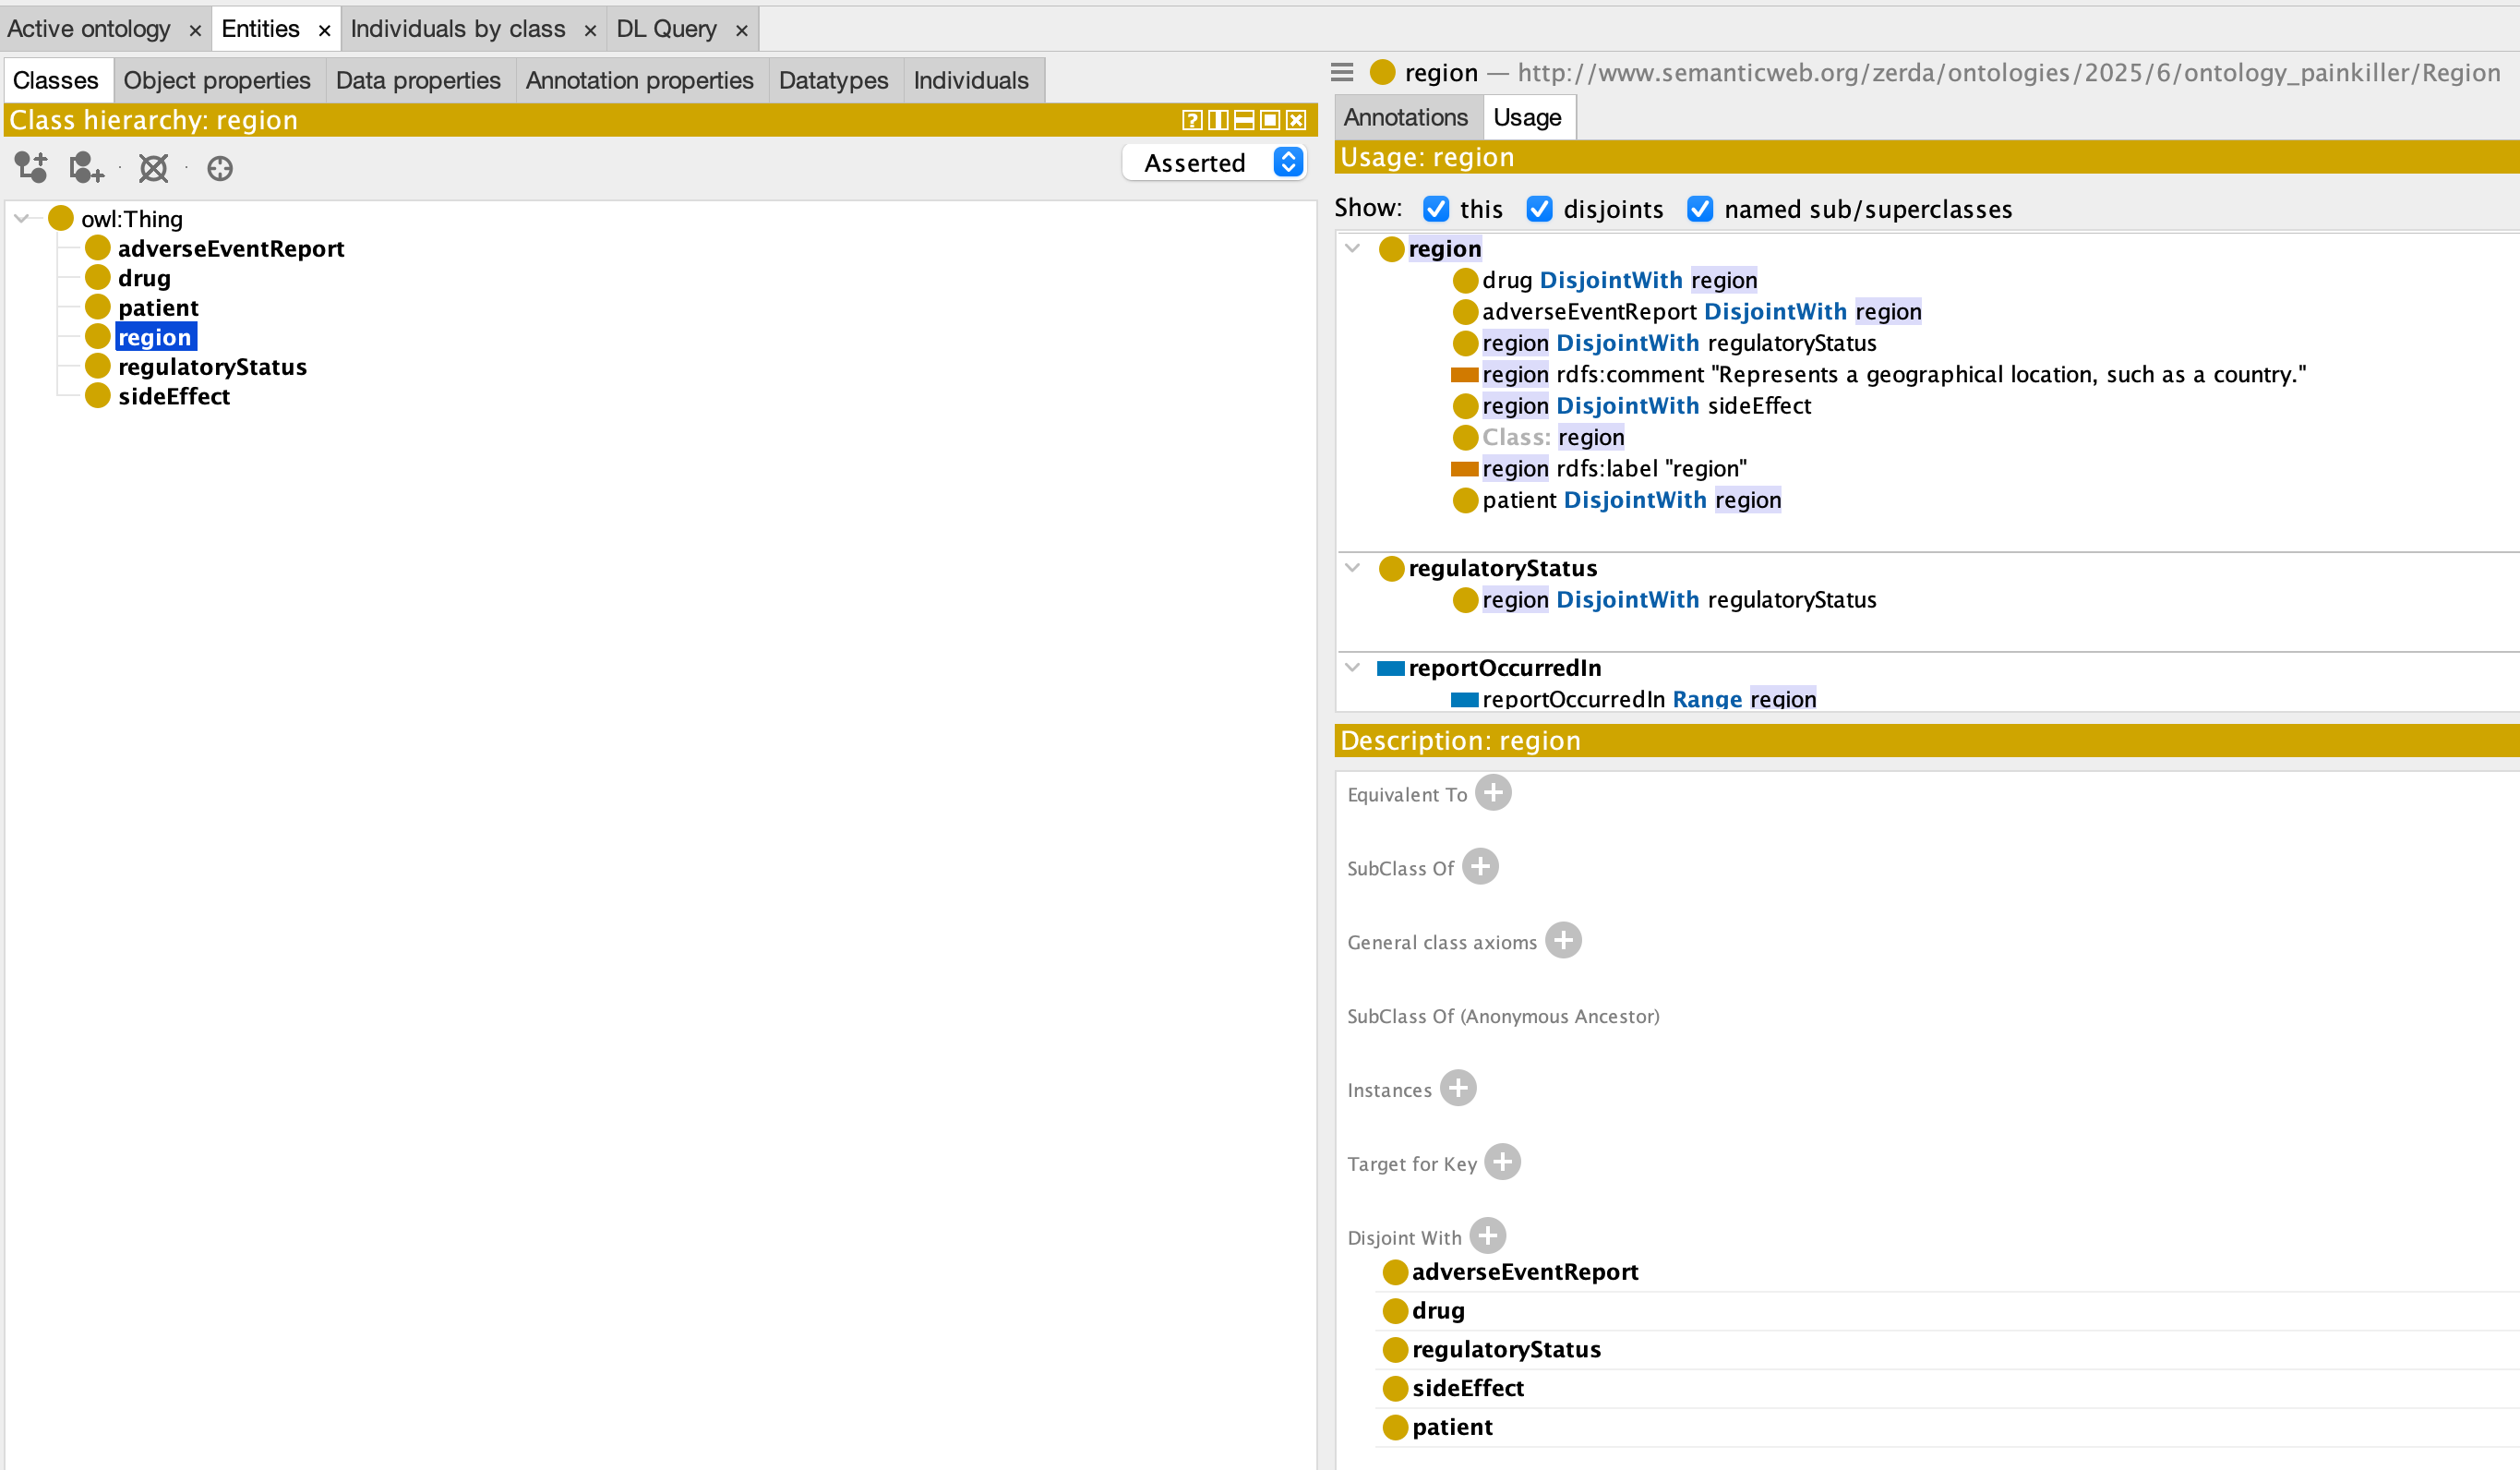
\includegraphics[width=0.9\textwidth]{pitfall_correction.png} % Replace with the path to your image
\caption{Protégé interface showing the added disjointness axioms.}
\label{fig:oops_correction}
\end{figure}

By addressing the “\texttt{missing disjointness}” pitfall, the ontology was significantly improved. Resulting in the final, validated scheme \nolinkurl{ontology_painkiller_after_oops.rdf} to be ready for the data population.

\subsection{Knowledge Graph Model and Population}
With the ontology schema now designed, refined and validated, the thesis now moves from the theoretical aspect to the practical implementation. This is how the model is brought to life with real-world data, so the schema can become functionally queryable. This section will now detail the final steps of this process: presenting the final conceptual model, mapping the prepared data into the RDF format and lastly loading it into GraphDB triple store to create the final artifact. 
\subsubsection{Final Conceptual Model}


In the final ontology the structure is normalized and relational, this is to represent all the nuances of the pharmacovigilance domain. This exact conceptual model was chosen for its flexibility, ability to separate real-world concepts into their own classes and semantic precision. What this does allow for is a clear and unambiguous representation, enabling complex, multi-part queries. The \texttt{AdverseEventReport} serves as the nexus of a central concept that connects \texttt{Drug}, \texttt{Patient} and \texttt{SideEffect}.

On a high level the final ontology schema is visualized in Figure~\ref{fig:vowl_visualization} using the Visual Notation for OWL Ontologies (\texttt{VOWL}), generated by the \texttt{WebVOWL} tool.The diagram illustrates the relationship between the core classes of the ontology. Thus showcasing the central roles of each and one of the classes.

\begin{figure}[H]
\centering
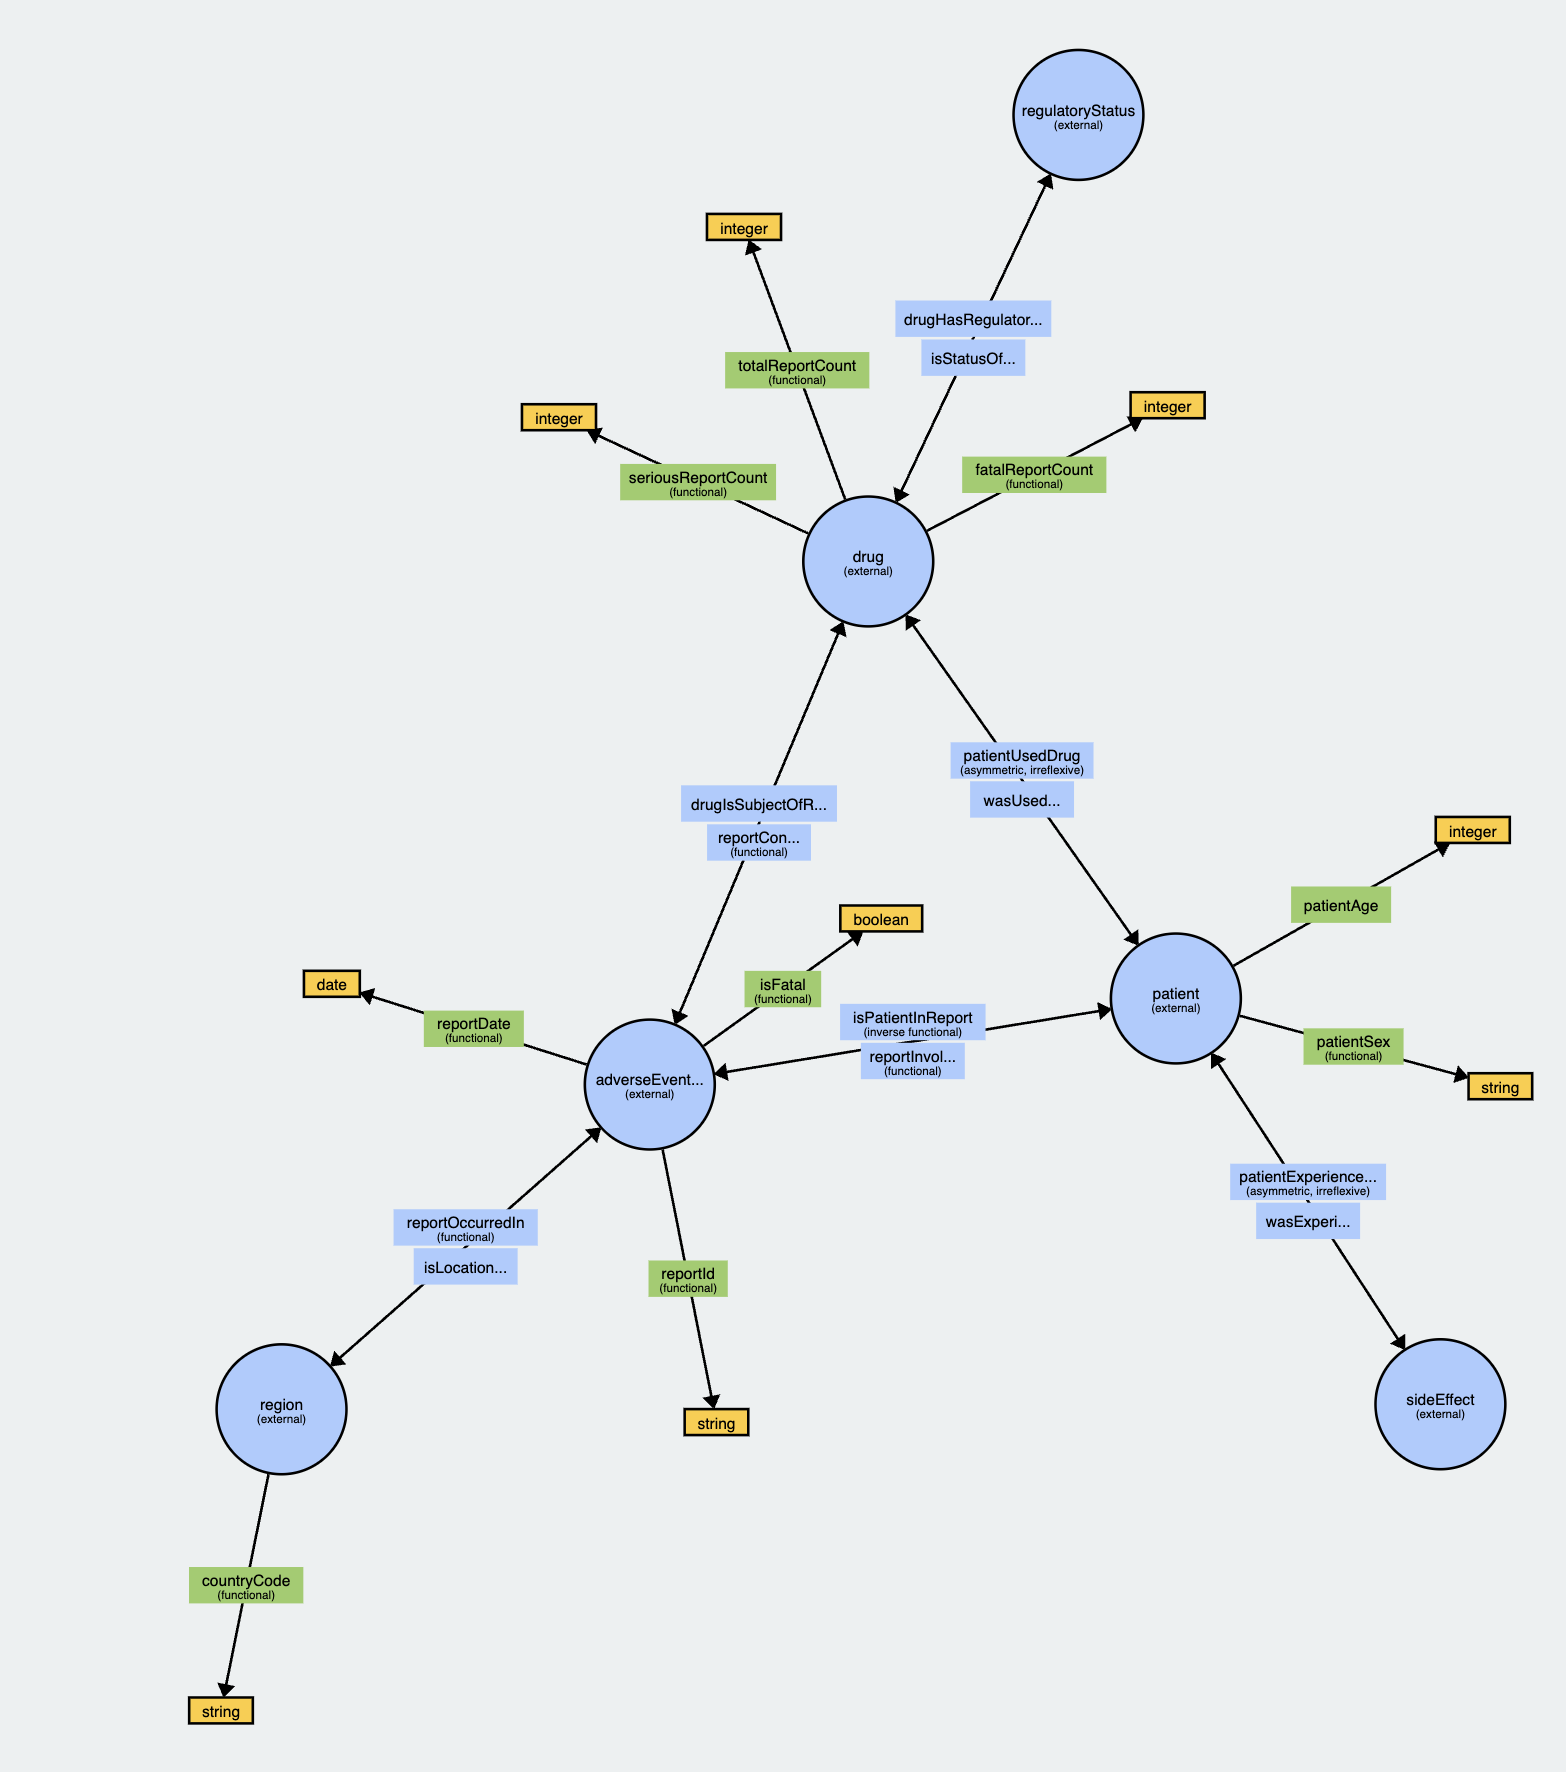
\includegraphics[width=\textwidth]{webvowl.png} % Replace with the path to your image
\caption{Visualization of the final ontology schema using WebVOWL.}
\label{fig:vowl_visualization}
\end{figure}

As illustrated in the diagram, the ontology is structured with several core classes serving as central nodes. The \texttt{Adverse\-Event\-Report} serves as a central concept that connects the \texttt{Drug}, \texttt{Patient} and \texttt{Side\-Effect} individuals. Thus ensuring that each piece of data is linked through the context of a real world report. This decision is crucial as it ensures that every fact is anchored to a specific documented event.

When looking at the relationships between the classes, we can see that they are defined by object properties. Which are for instance \texttt{report\-Concerns\-Drug}, which links an \texttt{Adverse\-Event\-Report} to the \texttt{Drug} individual that was the subject of the report. Similarly, when looking at \texttt{report\-Involves\-Patient} property, it links the same report to the unique \texttt{Patient}, who experienced the side effect of the drug. To ensure that the graph can be navigated in both directions, inverse properties such as \texttt{drug\-Is\-Subject\-Of\-Report} and \texttt{is\-Patient\-In\-Report} were added. Furthermore, making properties such as \texttt{report\-Involves\-Patient} functional, as it prevents data inconsistencies, since it enforces the rule that a single report can only involve one specific patient.

The clinical as well as demographic details are captured through the \texttt{Patient} and the \texttt{Side\-Effect} classes. A \texttt{Patient} is linked to a specific adverse event report, which they experienced through the \texttt{patient\-Experienced\-Side\-Effect} property. This is important, since it allows a many-to-many relationship. A single patient has the capability to experience multiple side effects, and a single side effect can therefore be experienced by many different patients. The attributes of the patient, such as \texttt{patient\-Age} and \texttt{patient\-Sex}, are also defined as data properties of the \texttt{Patient} class. This allows demographic analysis. Modeling \texttt{Side\-Effect} as its own class, rather than a simple test string, was another conscious decision. That way, side effects were no more attributes, but rather distinct entities, which are able to be aggregated and compared across the entire dataset. In this manner analytical queries about which adverse events were to occur most common, would be enabled.

The Geographic context is captured by the \texttt{Region} class. Each \texttt{Adverse\-Event\-Report} is linked to a \texttt{Region} through the \texttt{report\-Occured\-In} object property. The \texttt{Region} itself is described by a \texttt{country\-Code} data property. Thus allowing geographic analysis for the reports origin.

To complete the model, several other data properties were defined on the \texttt{Drug} and \texttt{Adverse\-Event\-Report} classes. The \texttt{Drug} class also included aggregated data from the openFDA API, such as \texttt{total\-Report\-Count}, \texttt{serious\-Report\-Count} and finally \texttt{fatal\-Report\-Count}. When we look at the \texttt{Adverse\-Event\-Report} it also contains details for each report such as a unique \texttt{report\-ID}, the \texttt{report\-Date}, a \texttt{report\-Country\-Code} and a boolean flag \texttt{is\-Fatal}, to confirm that each one of the reports were of patients who experienced a fatal death. The explicit use of data types such as \texttt{xsd:date} for \texttt{report\-Date} and \texttt{xsd:boolean} for \texttt{is\-Fatal}, allows the knowledge graphs query to further perform better calculations and operations.

Lastly, the regulatory context is also provided by the \texttt{Regulatory\-Status} class. Each \texttt{Drug} is linked to an individual from this class (e.g. “Over-the-Counter”) through the property \texttt{drug\-Has\-Regulatory\-Status}. This allows for an analysis, where drugs can be grouped based on their US legal status. Thus central to the risk-regulation paradox, which we are looking at here in this thesis.

\subsubsection{Knowledge Graph Population}
Thus central to the risk-regulation paradox, which we are looking at here in this thesis.

\subsubsection{Knowledge Graph Population}
The final step after validation is to populate the knowledge graph with instance data. This is also known as \texttt{RDF} mapping, which was performed using \texttt{Ontotext Refine}, which allows for transforming tabular data into a structured \texttt{RDF} format. The data from the initial \texttt{CSV} files was  transformed and refactored to fit the final, rich ontology model. This crucial step involved creating separate individuals for each \texttt{Drug}, \texttt{Adverse\-Event\-Report}, \texttt{Patient}, and \texttt{Side\-Effect}, and then generating the \texttt{RDF} triples that correctly link them together as defined by the object properties in the schema. This transformation resulted in a final set of three distinct Turtle (\texttt{.ttl}) files:
\begin{itemize}
    \item \nolinkurl{data_drugs.ttl}: Contains the individuals for each of the six painkillers, along with their data properties and regulatory status.
    \item \nolinkurl{data_reports.ttl}: Includes the individuals for each of the fatal \texttt{Adverse\-Event\-Report} instances.
    \item \nolinkurl{data_patients_effects.ttl}: Involves all the \texttt{Patient} and \texttt{Side\-Effect} individuals, which includes the demographic data and their links between patients and the side effects they experienced.
\end{itemize}
This section details the mapping process using the \nolinkurl{drug_risk_summary.csv} as an example. The \texttt{painkiller\_id} column serves as a basis for each \texttt{Drug} individual in the knowledge graph. The \texttt{total\_reports}, \texttt{serious\_reports} and \texttt{fatal\_reports} columns, contain the aggregated counts of different types of adverse event reports associated with each drug. The \texttt{marketing\_status} column contains the regulatory status of each drug.

\subsubsection*{Creating a Unique IRI}
The initial step included loading the \texttt{csv} file into a new \texttt{Ontotext Refine} project. But in order to create interconnected entities in the knowledge graph, we need to create a unique identifier before we go into the \texttt{RDF} mapping. So an Internationalized Resource Identifier (\texttt{IRI}) was established for each class. Thus allowing for different sources to be linked to it. As shown in Figure~\ref{fig:iri_creation}, this was achieved by combining the base \texttt{IRI} (\url{http://www.semanticweb.org/zerda/ontologies/2025/6/ontology_painkiller/}) with the value from the \texttt{painkiller\_id} column of the \texttt{CSV} (e.g. \texttt{Paracetamol}).

\begin{figure}[H]
\centering
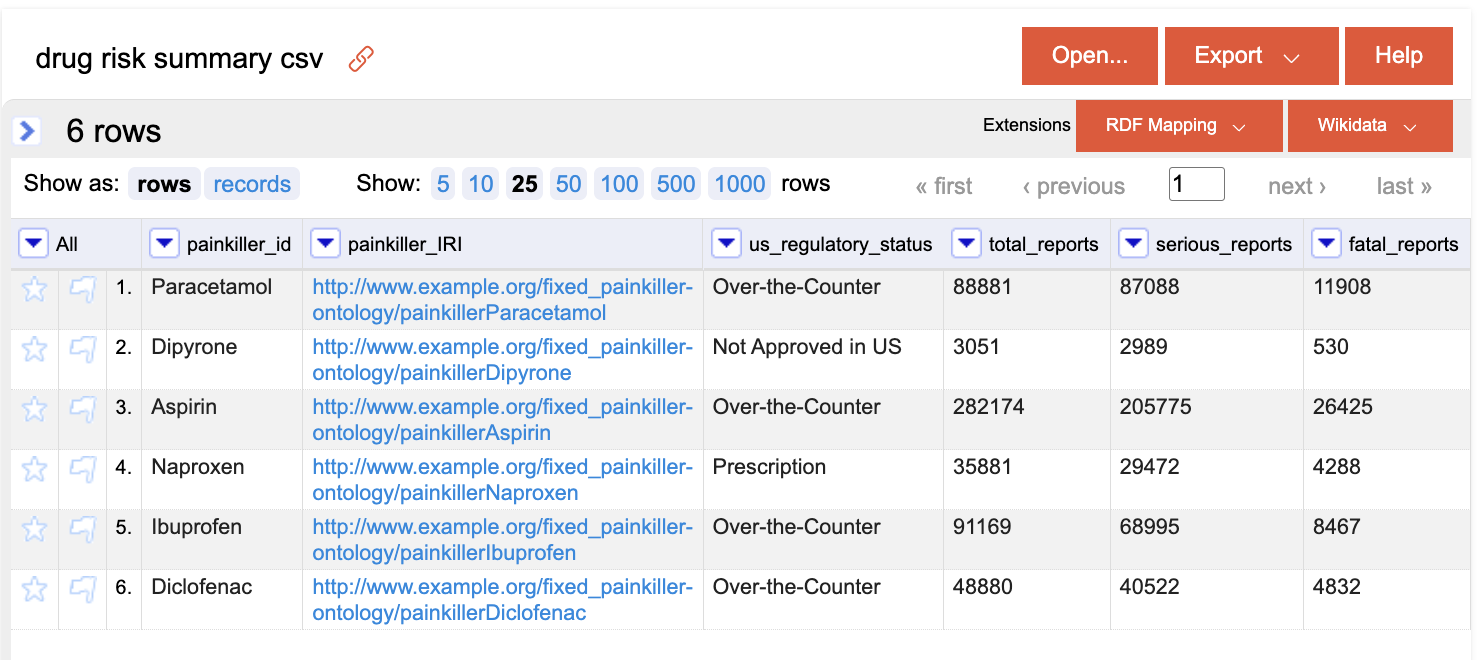
\includegraphics[width=0.9\textwidth]{ontotext_refine_example.png} % Replace with the path to your image
\caption{Creating a unique IRI in Ontotext Refine.}
\label{fig:iri_creation}
\end{figure}

\subsubsection*{Mapping Data to Properties}
Now all that was left is to map each column to its corresponding property. Figure~\ref{fig:mapping_process} illustrates this process. As a starting point, each row in the table is identified as an instance of \texttt{wu:Drug}, with “\texttt{wu}” being a prefix for the base \texttt{IRI}. The base acts as a root namespace. The aggregated data is mapped to its corresponding data properties, for example the \texttt{total\_reports} column is mapped to \texttt{wu:total\-Report\-Count}, linking each drug to its total report count attribute. This pattern is used for each data property. The \texttt{marketing\_status} is mapped to the \texttt{wu:drug\-Has\-Regulatory\-Status}, which links the \texttt{Drug} individual to the \texttt{Regulatory\-Status} individual.

During the mapping process, it is also crucial to specify the correct data type so that it is machine-readable and can be used in further calculations. The value from the \texttt{fatal\_reports} was therefore defined as an \texttt{xsd:integer}, which created a typed literal in the knowledge graph. Thus allowing \texttt{SPARQL} to perform mathematical operations, such as calculating averages or percentages. This approach was used for all other aggregated report counts. For the other columns, their value was defined as a literal with a language tag (\texttt{@en}),  so that the data can be interpreted correctly.
Once the mapping was complete, the data was exported from \texttt{Ontotext Refine} as the turtle file \nolinkurl{data_drugs.ttl}. Thus process what repeated for all datasets, so all instances can now be queried and analyzed.

\begin{figure}[H]
\centering
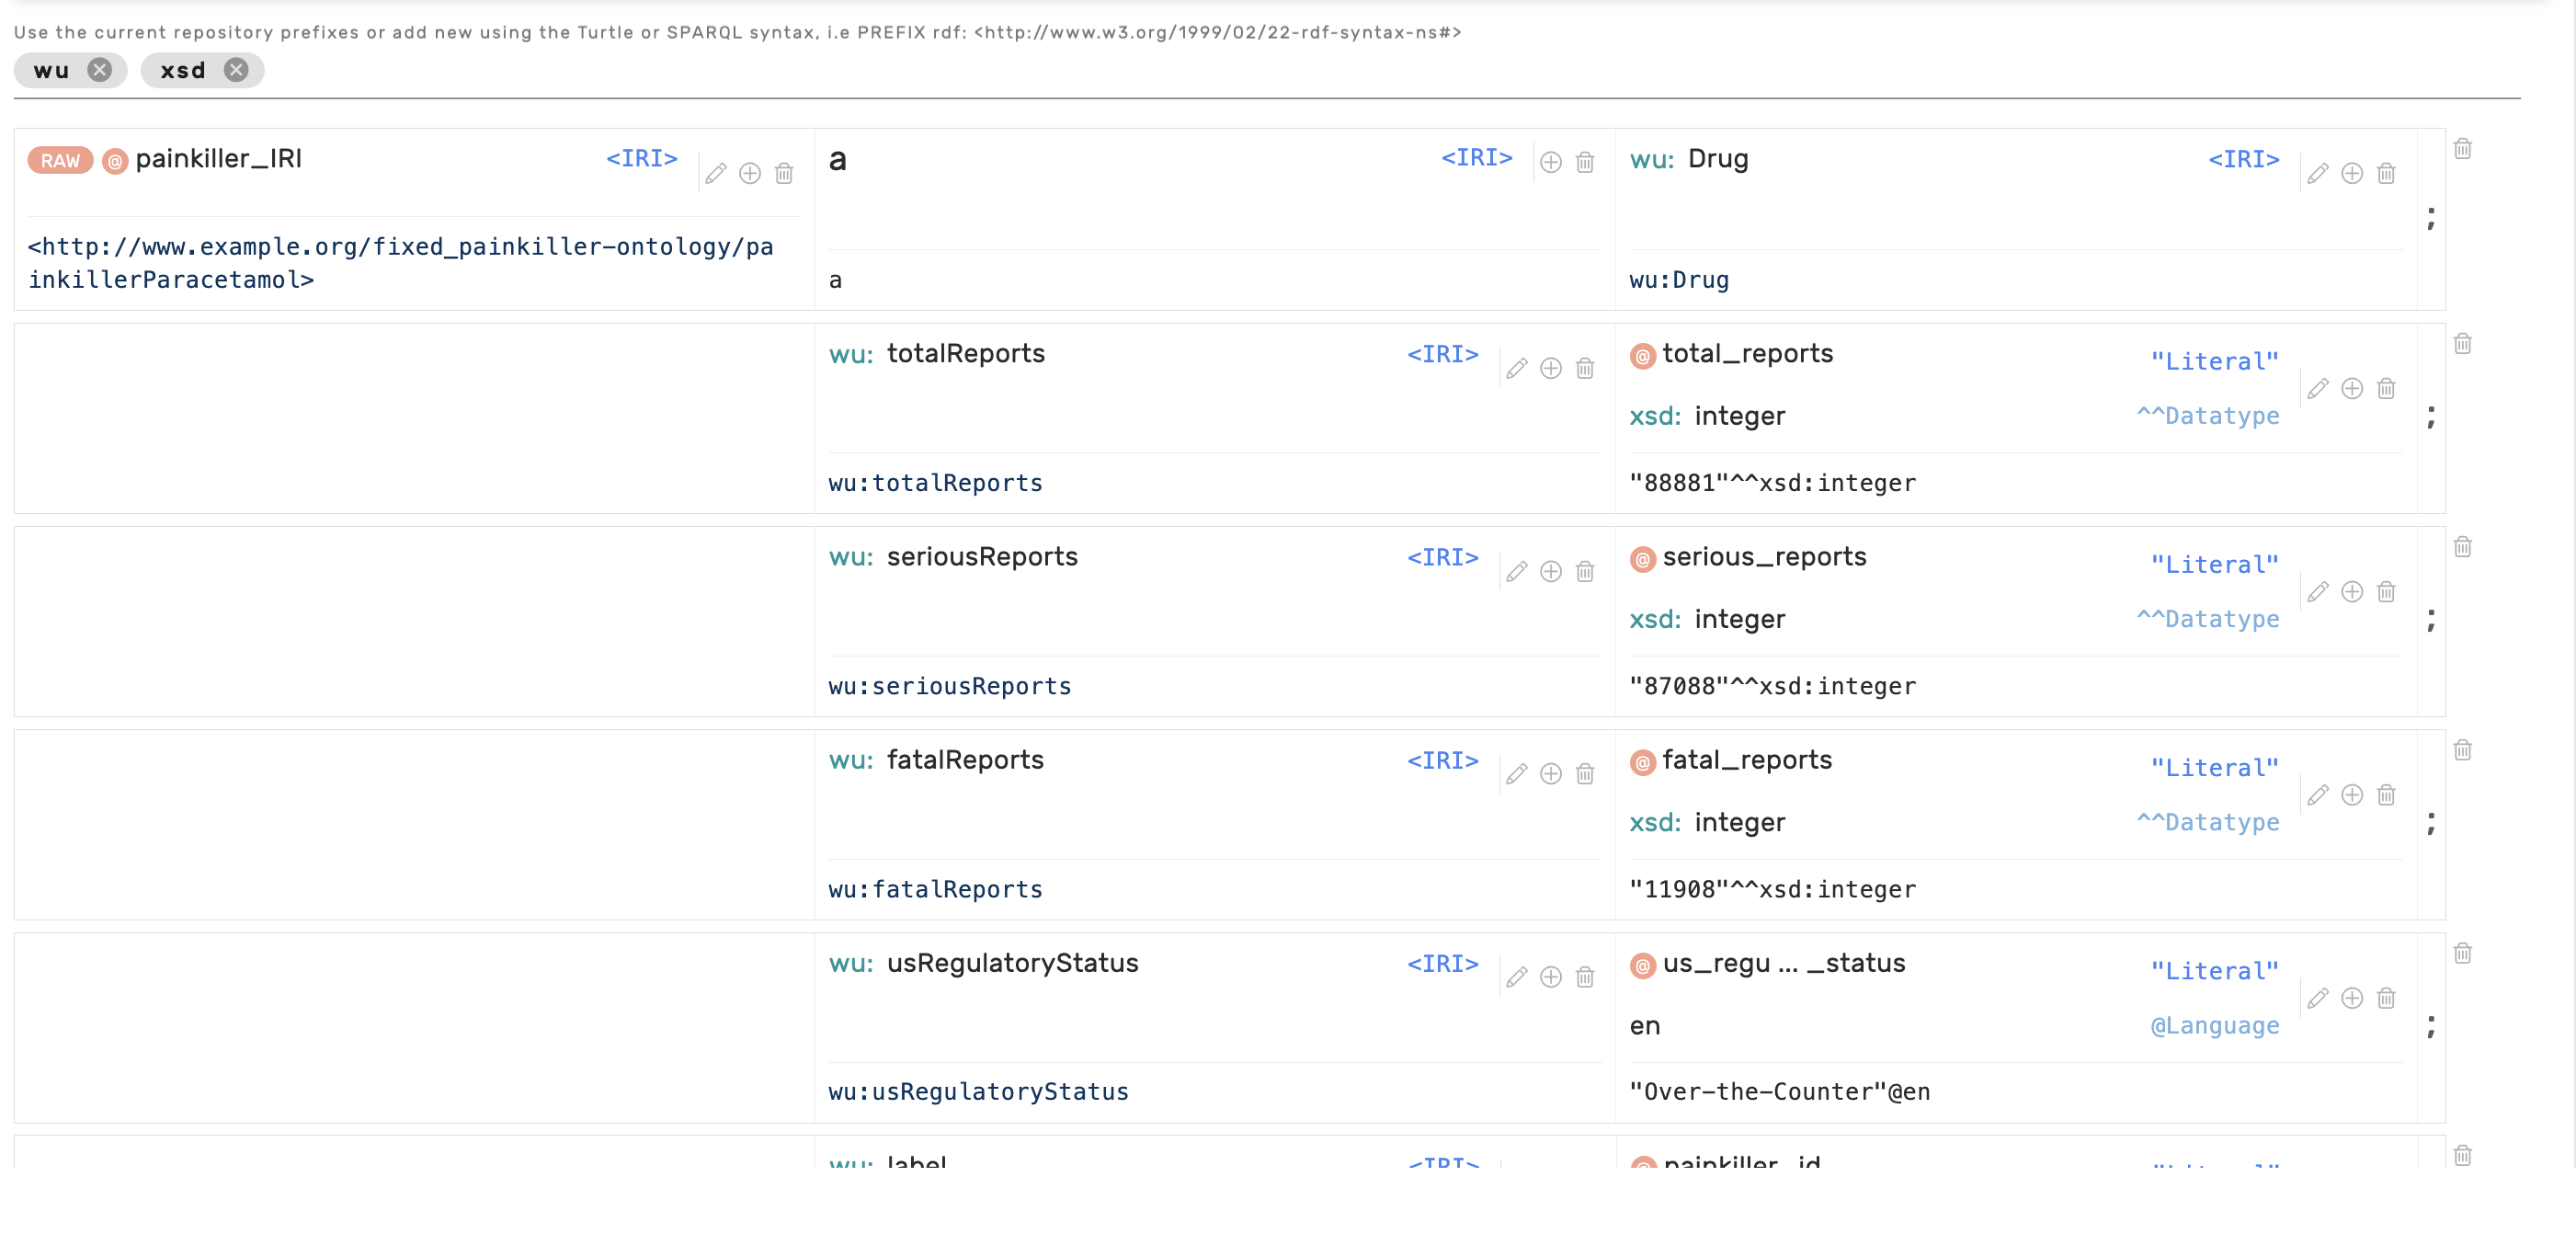
\includegraphics[width=\textwidth]{mapped_example.png} % Replace with the path to your image
\caption{Mapping columns to properties in Ontotext Refine.}
\label{fig:mapping_process}
\end{figure}

\subsubsection*{Loading into GraphDB}
These final \texttt{.ttl} files were then loaded into a \texttt{GraphDB} triple store. \texttt{Ontotext GraphDB} is a powerful and scalable graph database that allows for the storage, management, and querying of \texttt{RDF} data. Loading the data into \texttt{GraphDB} transformed the separate files into a single, unified, and queryable knowledge graph. Figure~\ref{fig:graphdb_hierarchy} shows the final class hierarchy as displayed in the \texttt{GraphDB} interface. As shown, the final model consists of five primary classes.

\begin{figure}[H]
\centering
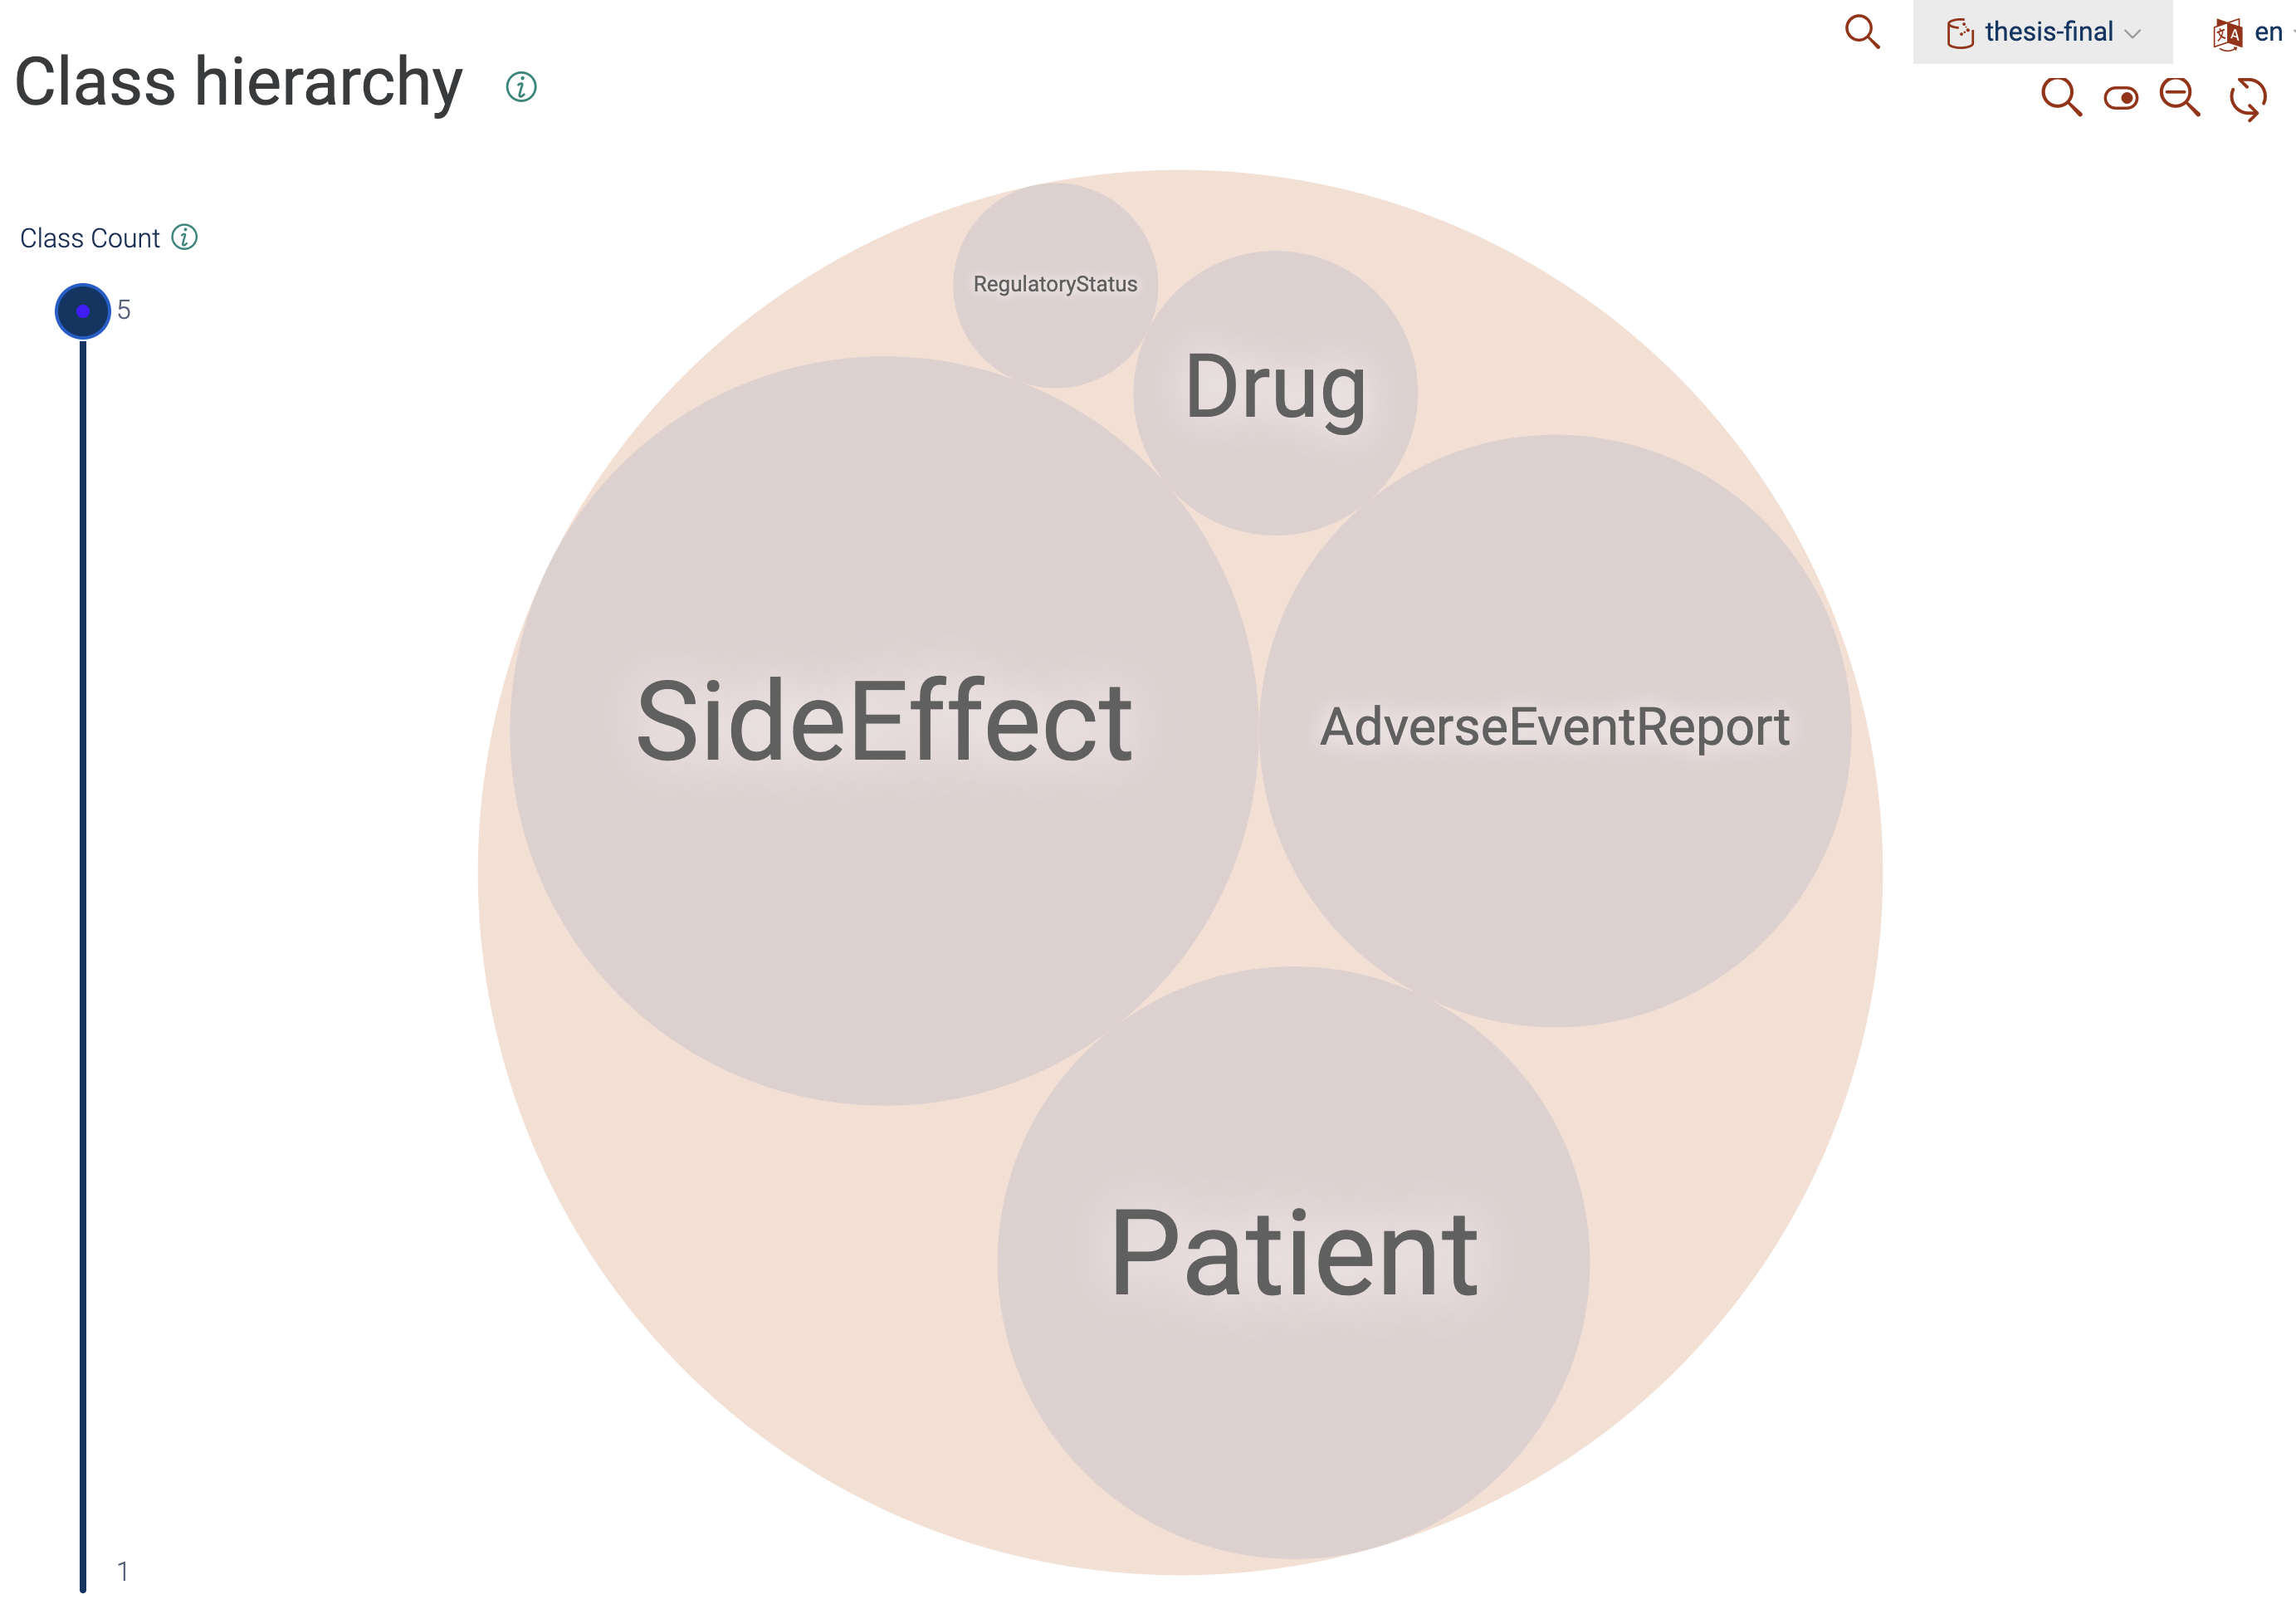
\includegraphics[width=0.8\textwidth]{final_class.png} % Assumes SVG was converted to PNG
\caption{Final class hierarchy as displayed in GraphDB.}
\label{fig:graphdb_hierarchy}
\end{figure}

The number or individuals or instances in each class reveals the expected distribution. \texttt{Side\-Effect} has the highest instance count, which makes sense because a small number or reports can describe a variety of medical events. \texttt{Adverse\-Event\-Report} and \texttt{Patient} are the next largest classes.
\texttt{GraphDB}'s visual interface provides an important tool for verifying that the data has been loaded and linked correctly according to the ontology's schema. The visualization allows for an intuitive exploration of the relationships between different individuals, such as confirming that specific \texttt{Adverse\-Event\-Report} instances are correctly linked to the \texttt{Drug} and \texttt{Patient} individuals they concern.

\section{Evaluation}

This chapter evaluates the functional capabilities of the painkiller ontology. The primary method to evaluate is to test the now populated ontology against the competency questions, by executing a series of \texttt{SPARQL} queries. Each query's result is presented and interpreted to demonstrate that the knowledge graph can show insights about the data. 
To maintain focus in this thesis, only the most insightful queries will be presented in full. The complete set of all queries developed for this analysis is available in the public GitHub repository in the \texttt{/queries} folder.

\subsection{Initial Side Effect Retrieval}
The initial evaluation validates if the ontology is able to answer foundational questions to begin with. Therefore, the focus on a single drug, Ibuprofen, was deemed as fitting to demonstrate a simple data retrieval operation.
A basic query \nolinkurl{1_list_side_effects_for_drug.sparql} was run to confirm if the ontology could answer the competency question: “Which side effects are associated with Ibuprofen?”. The query successfully retrieved a list of all the side effects and could validate the structure of the graph, nonetheless a simple side effect list does not reveal which conditions are reported most frequently. To further narrow down the scope and to address the limitations of the first query, the follow up query \nolinkurl{2_count_side_effect_frequency.sparql} was constructed to count if there were side effects that occurred more than once, when using said drug. In this instance, the outcome revealed that ``\texttt{Renal failure acute}'' and ``\texttt{Toxicity to various agents}'' were the most frequently reported conditions for Ibuprofen in this dataset, to highlight recurring events.

While this can be useful, when looking at the side effects of each drug individually, it would be more useful to see everything at once, in order to go through a comparative analysis across the entire dataset. Therefore the following query: \nolinkurl{3_list_side_effects_all_drugs.sparql} showed all of the side effects at once and \nolinkurl{4_count_side_effects_all_drugs.sparql} narrowed it down again by showing which side effect occurred more than once for each drug. A visualization of the query can be seen in Figure~\ref{fig:query4_visualization}, and the corresponding results table is shown in Figure~\ref{fig:query4_results}.

\begin{figure}[H]
\centering
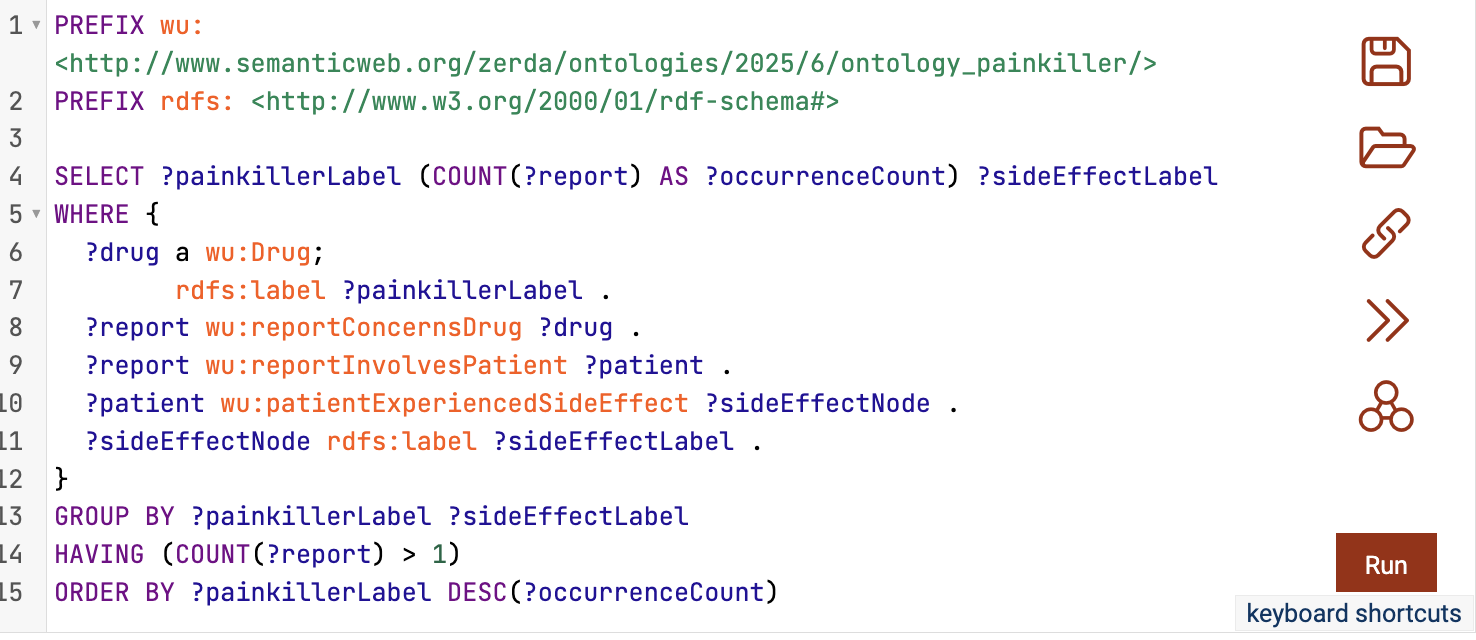
\includegraphics[width=\textwidth]{query_example.png} % Replace with the path to your image
\caption{Visualization of the SPARQL query for counting recurring side effects.}
\label{fig:query4_visualization}
\end{figure}


The query’s \texttt{WHERE} clause constructs a path through the ontology to link each painkiller to its reported side effects:
First, \nolinkurl{?drug a wu:Drug; rdfs:label ?painkillerLabel .} will look for all the individuals that are of the type \texttt{wu:Drug} and takes their name through the \texttt{?painkillerLabel} variable.
Then \nolinkurl{?report wu:reportConcernsDrug ?drug .} creates the first link, while finding tall \texttt{Adverse\-Event\-Report} individuals that are associated with each drug. \nolinkurl{?report wu:reportInvolvesPatient ?patient .}, looks for the \texttt{Patient} individual that is linked to each report. This is then completed with \nolinkurl{?patient wu:patientExperiencedSideEffect ?sideEffectNode .} and \nolinkurl{?sideEffectNode rdfs:label ?sideEffectLabel .}, which together find the specific \texttt{Side\-Effect} individuals for each patient as well as retrieving their names.

After all the links are built  \nolinkurl{GROUP BY ?painkillerLabel ?sideEffectLabel} aggregates the results. This creates a separate group for each combination of a drug and side effect. \nolinkurl{HAVING (COUNT(?report) > 1)} then filters these groups, making sure that only the side effects that have been reported more than once for a specific drug are included in the final result.
To finish this off \nolinkurl{ORDER BY ?painkillerLabel DESC(?occurrenceCount)} sorts the results. The query then gives us the results table, which reveals that for Naproxen, the side effect “Toxicity to various agents” was reported 9 times in separate fatal cases. Thus marking it the most frequently reported adverse event for any drug in the dataset. This demonstrates that the knowledge graph can surface significant risk patterns and the use of being a potential safety signal for this specific drug, which allows for further investigation.

\begin{figure}[H]
\centering
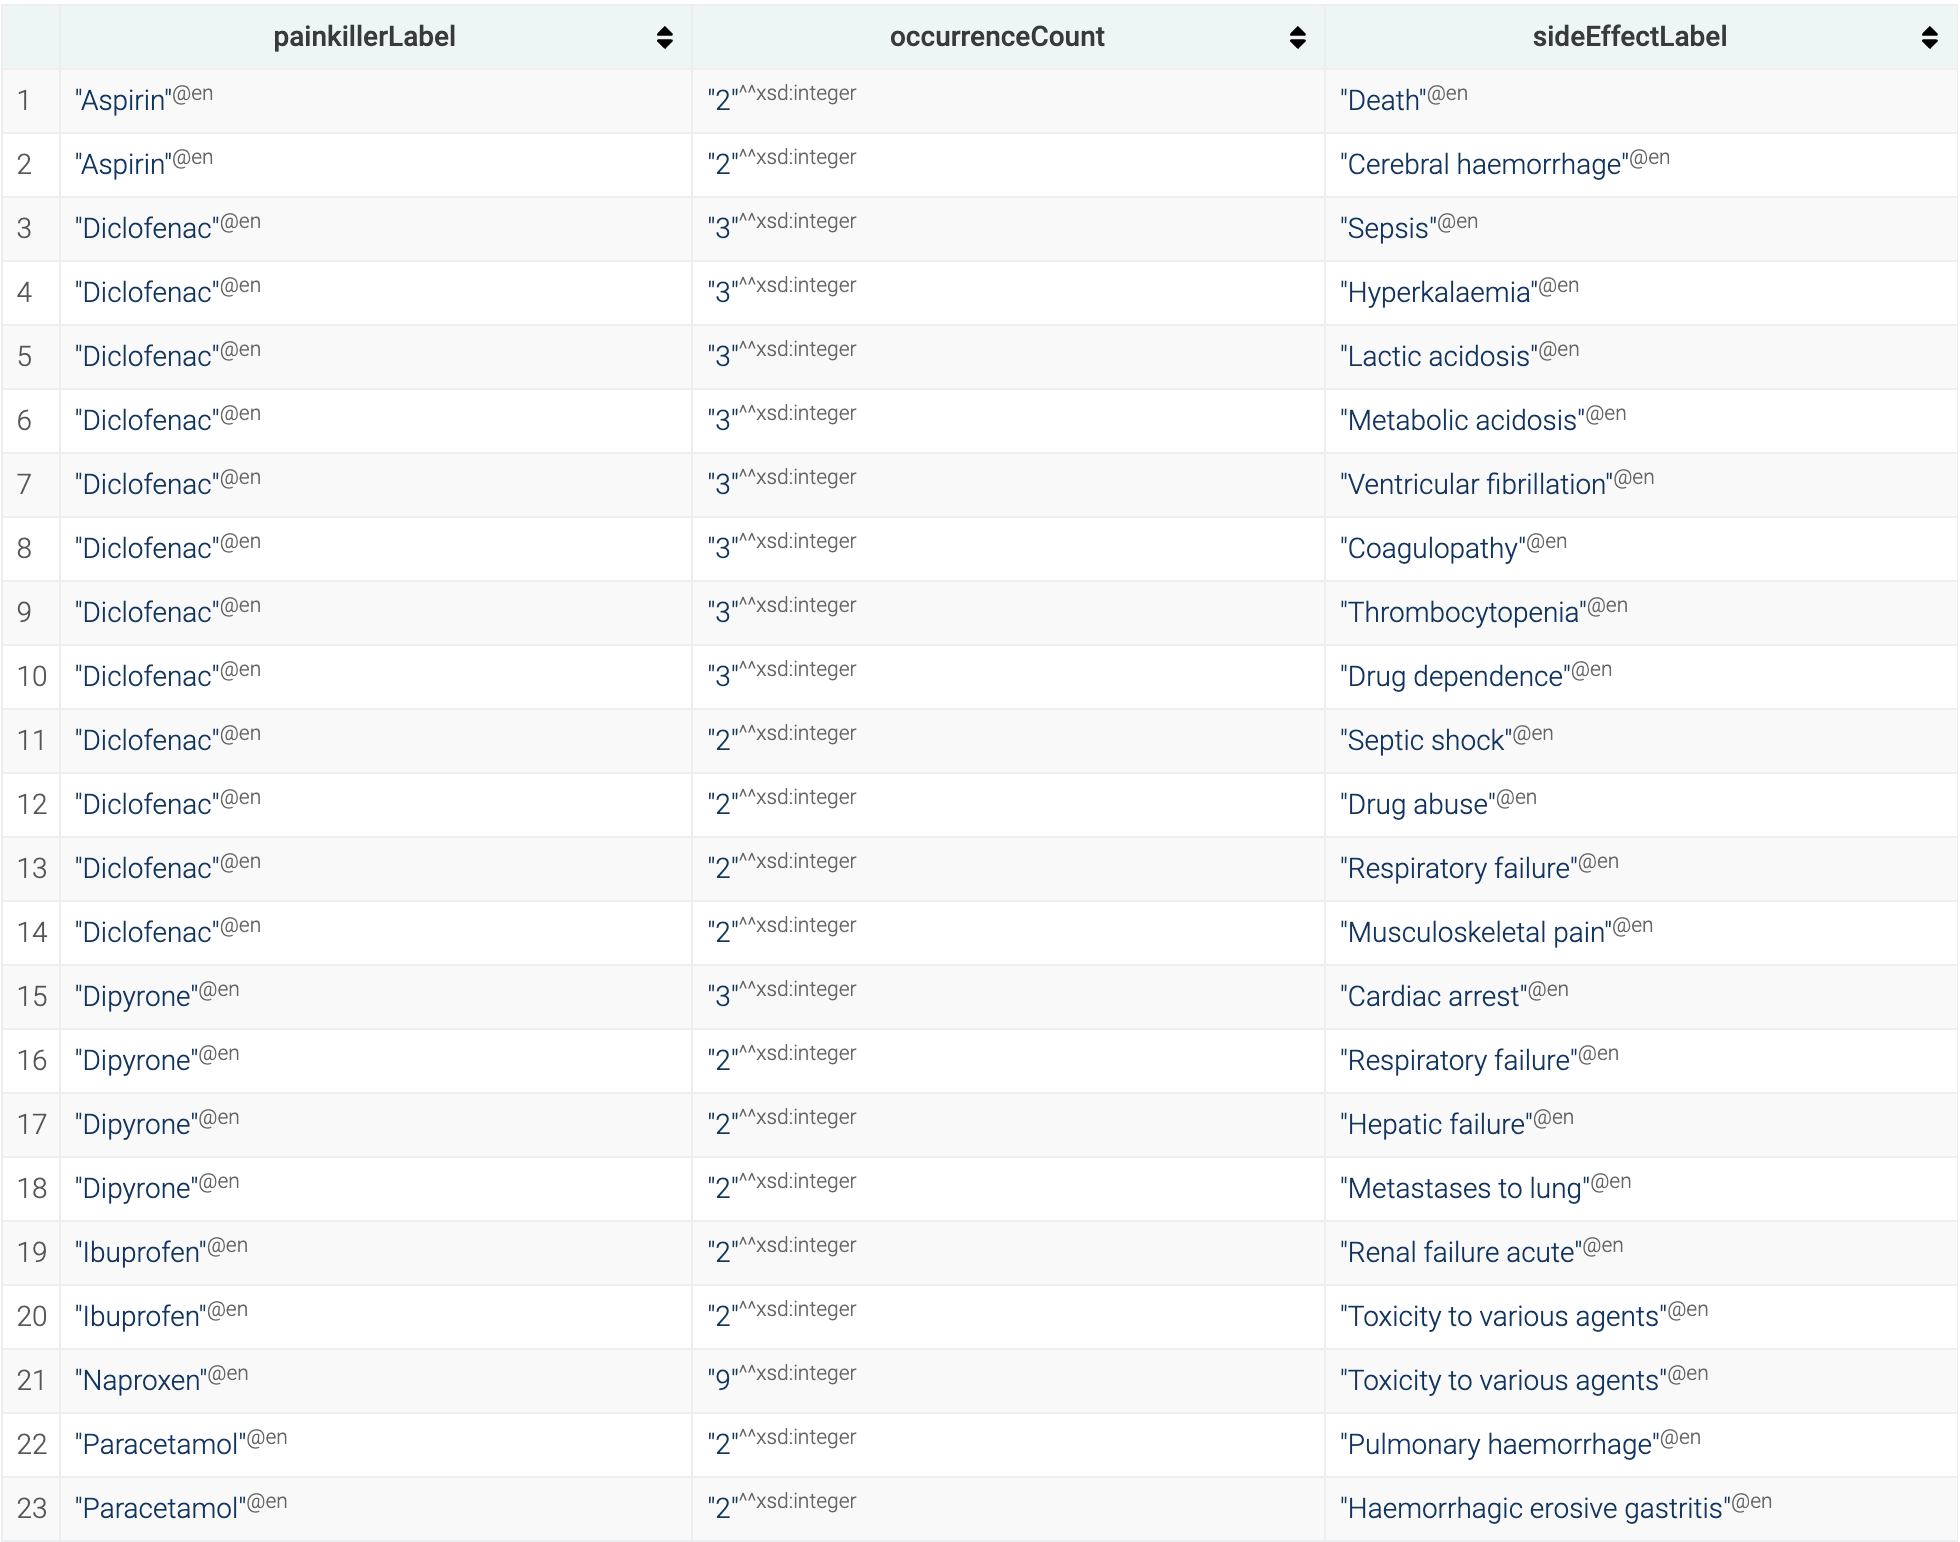
\includegraphics[width=\textwidth]{query_result1.png} % Replace with the path to your image
\caption{Results of counting recurring side effects for all drugs.}
\label{fig:query4_results}
\end{figure}

\subsection{Demographic and Regulatory Analysis}
The next query \nolinkurl{5_avg_patient_age_by_drug.sparql} expands the analysis to patient demographics by calculating the average age of patients in fatal reports for each painkiller. One of the key findings is that there is a strong association between Aspirin and an elderly demographic. To be more exact, Aspirin was associated with the highest average patient age at 72 years. Contrasting that, when looking at Dipyrone, the average age was 47. Thus allowing for a more nuanced discussion, where the argumentation holds that the fatal report percentage is not just the whole story and the demographic context of that risk is just as important.

To investigate the risk regulation paradox in one go, the \nolinkurl{6_avg_risk_by_regulatory_status.sparql} query was created. Here instead of comparing the individual drugs, the query groups all painkillers by their regulatory status and calculates the average fatal report percentage as a result. Therefore when ignoring all other aspects, we can just plainly compare whether “Over-the-Counter”, “Prescription” or “Not Approved in US”, really have a difference in their fatality outcome. As a result,  “Not Approved in US” drugs did show the highest risk profile with 17.37\%. Another finding resulted that the OTC drugs had a similar fatality percentage as the prescription based drugs of around 10\%.

\subsection{Geographic and Multi-dimensional Analysis}
Another way to query would be to look if there is a correlation between the geographic location and the patient age to analyze the date. This is precisely done in \nolinkurl{9_analyze_metaminzole_reports.sparql}. The idea was to see if the country played a role in the fatality outcome. This reasoning stems from the fact that not every country offers the same healthcare system as the one we have in Austria. Some people need to pay out of pocket for each hospital visit, which can be unaffordable for portions of the population. So for this query the drug Metamizole (known as Dipyrone in the U.S.) was taken into consideration as a test run. The results show most of the reports were from Brazil, where the patients were mostly elderly. This could help in concluding and trying to research more into the possibility, whether or not there is poverty in old age in said country.

To further expand this analysis on the geographic location the query \nolinkurl{10_insert_multi_dimensional_risk_analysis.sparql} was created to provide a comprehensive, multi-dimensional view of the drug risk, considering the possibility to uncover the complex interplay between a drug’s risk, its regulatory status and the specific demographic and geographic contexts in which those fatal events occurred.



The results in Figure~\ref{fig:multidim_results} from this final \texttt{SELECT} query revealed what we already knew about Dipyrone: it has the highest fatal report percentage, and it is paired with the regulatory status “Not Approved in US”, but it now also puts into perspective that 60\% of these fatal reports originated from Brazil with the average patient age of 58. This single country therefore contributes the 10.42 percentage points to the total risk figure, meaning that the majority of statistical risk is concentrated in this one region.
Another finding is that Paracetamol (Tylenol in the U.S.), an OTC drug, shows a significantly higher fatal report percentage than both Ibuprofen and the prescription drug Naproxen. Worth mentioning would be the geographic locations, of which Paracetamol risk in this dataset is concentrated in the reports from the United Kingdom, while the Ibuprofen risk is in the United States and Naproxen's outcome also stems exclusively from the latter. This could lead to the assumption that prescription drugs have a higher risk percentage than OTC drugs.

\begin{figure}[H]
\centering
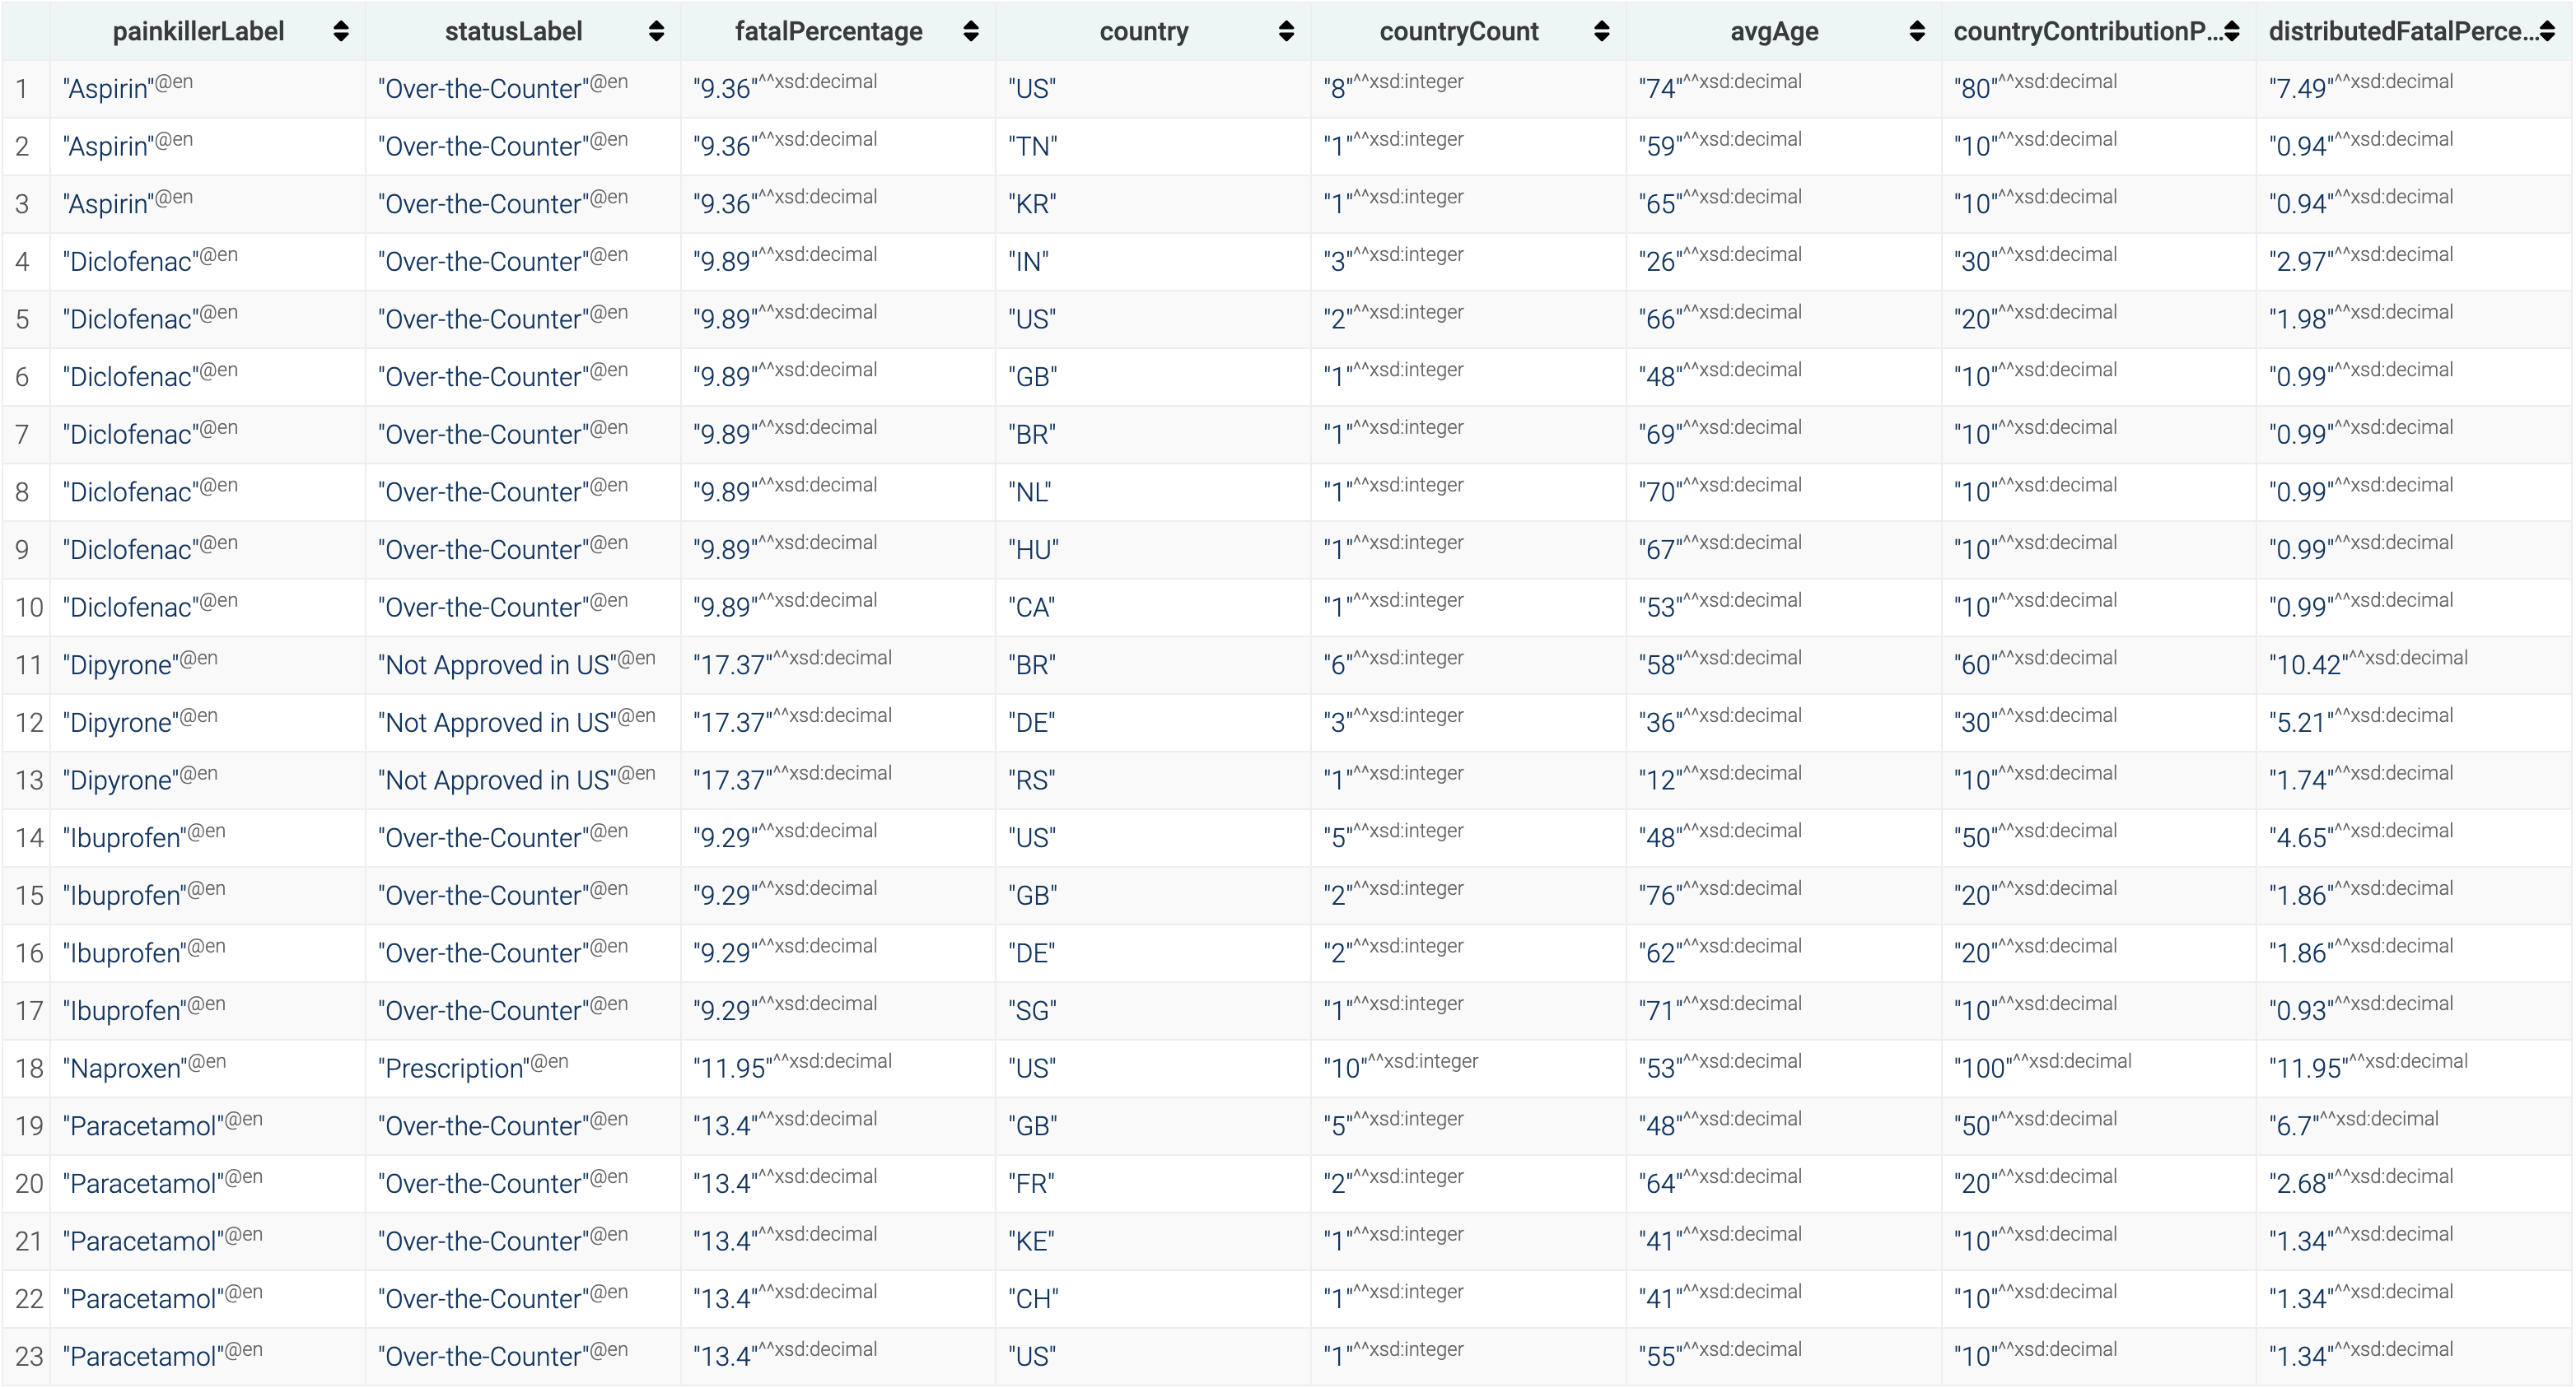
\includegraphics[width=\textwidth]{multidimensional_risk_analysis.png} % Replace with the path to your image
\caption{Results of the multi-dimensional risk analysis query.}
\label{fig:multidim_results}
\end{figure}

Now that we know that most fatal reports for Dipyrone originated from Brazil, another question could be asked: "Within this Brazilian hotspot, are there any specific side effects that are reported more frequently than others?". The query that looks at this question is \nolinkurl{14_geographic_hotspot_analysis.sparql}. So it looks at the reports concerning Dipyrone that originated in Brazil and then calculates the frequency of each side effect within that subset. As a result the side effects which were the most common were ``\texttt{Cardiac arrest}'' (3 times), then ``\texttt{Respiratory failure}'' and ``\texttt{Metastase to lung}'' (2 times each). After this query it allows us to see beyond Brazil just having the highest number of reports, to know that fatal reports for Dipyrone in Brazil in this dataset are associated with severe cardiovascular and respiratory events. This shows that we can dive even deeper within the analysis of this knowledge graph.

\subsection{Demographic Correlation with Side Effects}
However this raises another question: “Is the age difference a property of the drug itself, or is it related to the specific types of fatal side effects that are being reported?” To investigate this hypothesis, the query \nolinkurl{11_side_effect_demographic_correlation.sparql} was developed. This time not grouping by the drug, but rather flipping the narrative by grouping by side effect. By calculating the average age of patients for each side effect as well as the patient count,  this query allows us to see if there is a specific side effect that is more prevalent in certain age groups, regardless of what drug was in use. While ``\texttt{Cerebral haemorrhage}'' had the highest average age of 86, it was only reported in 2 patients. In stark contrast, the most frequently reported fatal side effect is ``\texttt{Toxicity to various agents}'', which was reported in 11 separate patients with the average age being 47. This could mean that those people might have died from an overdose, which can be attributed to drug abuse, rather than saying that the drug itself was the problem.  Another finding was that side effects such as ``\texttt{Hyperkalaemia}'', ``\texttt{Lactic acidosis}'' and ``\texttt{Drug dependence}'' were all associated with an average patient age of 26. This prompts the follow up question “Which specific painkiller is associated with this cluster of life-threatening side effects observed in the young adult patient group?”.

\begin{sloppypar}
To answer this question the following query \nolinkurl{12_drug_analysis_for_young_toxicity_profile.sparql} was executed. For this the following terms were included within the filter of the query:``\texttt{Hyper\-kalaemia}@en'', ``\texttt{Lactic acidosis}@en'', ``\texttt{Thrombo\-cyto\-penia}@en'', ``\texttt{Ventricular fib\-ril\-lation}@en'', ``\texttt{Drug dependence}@en''.  As a result the toxicity-related side effects observed in young adult patients were exclusively associated with Diclofenac in this dataset. This indicated a probable result of overdose or misuse.
\end{sloppypar}

Having now looked at the young adult toxicity profile, the next logical step would be to perform the same drill for the elderly profile, where we could look at their frailty. The initial demographic analysis revealed that the side effect ``\texttt{Cerebral haemorrhage}'' was what was associated with the highest average patient age. This begs the question “Which specific painkiller is most frequently associated with “Cerebral haemorrhage” in this elderly patient group?”. For which the query \nolinkurl{13_drug_analysis_for_elderly_haemorrhage_risk.sparql} was created. The query reveals that the two patients had been taking Aspirin in our dataset, with the average age being 86. The risk of Cerebral haemorrhage (bleeding in the brain) is a known risk associated with Aspirin, which increases with age. Those types of queries can work as a real life checker, to see whether the facts uphold within healthcare specialists.

\subsection{Temporal and Gender-Based Analysis}
Now to also understand the evolution of the drug safety reporting over time within the dataset, this query was created \nolinkurl{15_temporal_trend_analysis.sparql}.  Here each year got extracted from each report's date, and then the reports were grouped by year and by the painkiller itself. As well as a count of how many fatal reports were filed each year for each drug. This created the following table in Figure~\ref{fig:temporal_trend_results}.

\begin{figure}[H]
\centering
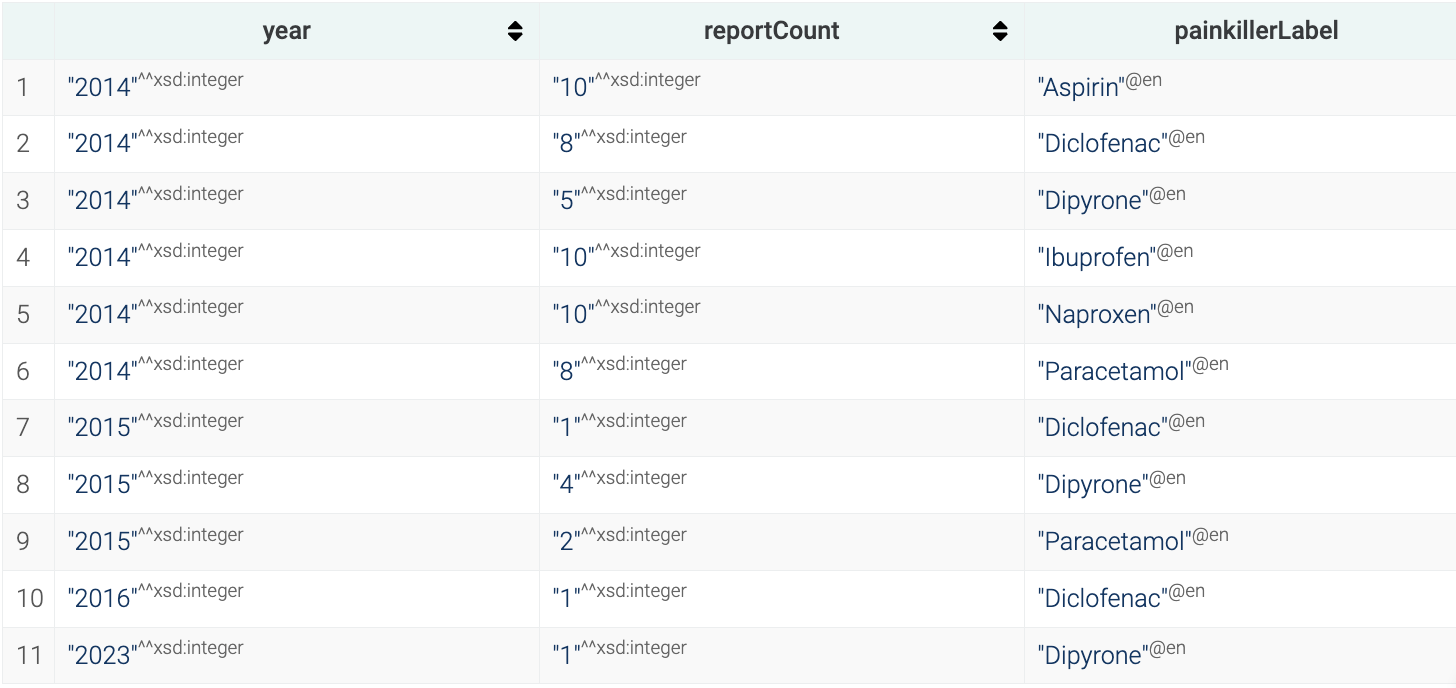
\includegraphics[width=0.9\textwidth]{temporal_trend_results.png} % Replace with the path to your image
\caption{Temporal distribution of fatal adverse event reports by drug.}
\label{fig:temporal_trend_results}
\end{figure}


This query now revealed that there is a heavy concentration of data in 2014. While there are also reports from 2015 and a few outliers in later years, the data is not distributed evenly. For both Naproxen and Ibuprofen the reports exclusively took place in 2014. This is worth mentioning because it shows that the dataset is just a snapshot and not complete. It also raises the question whether the amount of fatal reports diminished over time since medicine can drastically change over the years, with better equipment and also better ways to help people survive.

The previous analysis revealed the characteristic that the reports are heavily concentrated in the year 2014. However, since some drugs, like dipyrone, have fatal reports spanning over more years than one, this opted for the following question “For Dipyrone, did the demographic profile of the patients in fatal reports change over time?” This query \nolinkurl{8_longitudinal_demographic_profile.sparql} was created. This query produced a small table, but still worth mentioning. It revealed a clear downward trend in the average age of patients involved. The average age experienced a drop from 53 in 2014 to 46 in 2015 and lastly with the most recent report in 2023 involving a 16 year old. Now what does that mean? This could potentially mean that there are risk factors in younger patients when using this drug.

To investigate the role of the patient demographics in fatal adverse events, the query \nolinkurl{16_gender_distribution_analysis.sparql} was designed to analyze the gender distribution of reports for each painkiller medication. Here the query will group all reports by the drug and the patient's sex and then the number or reports will be counted. The results for this query revealed that the gender distribution is not uniform across all drugs. This could suggest that gender may also be a variable in the risk profiles of the painkillers. For instance, when looking at aspirin, the fatal reports were twice as common in males (7 times) than in females (3 times). When looking at dipyrone, the trend is reversed, where the females fatal reports are more common than in males.  This could suggest that when prescribing drugs the gender should also be taken into consideration. So there isn't really a one size fits all approach.

Just now we saw that there was a gender skew in the fatal reports for Dipyrone, for this case we can also dive deeper with the following question: “Are the types of fatal side effects reported for Dipyrone different for females versus males?”. This was evaluated through this query \nolinkurl{17_gender_based_side_effect_profile.sparql}.

This query focuses only on one drug and generates a frequency count of each side effect, which is broken down by the gender of the patient. Now this result table reveals that \texttt{Hepatic failure}, \texttt{Cardiac arrest} and \texttt{Metastases to lung} are each reported in 2 separate cases for females. As well as the side effects ``\texttt{Toxic epidermal necrolysis}'' and ``\texttt{Stevens-Johnson syndrome}'', which could be strong indicators that especially females are at risk when taking Dipyrone, when it comes to liver and heart failure. Thus concluding that males experienced less risk, since their side effects were not once reported more than once.


\section{Discussion and Conclusion} 
In this thesis, the focus is to design and implement a knowledge graph for analyzing fragmented pharmacovigilance data using semantic technologies. The results of the evaluation using this knowledge graph were presented in Chapter 4. This final chapter puts these results into perspective and links them with the research questions RQ1, RQ2, and RQ3.

First, Section 5.1 presents the results with regard to each research question. Second, Section 5.2 outlines the key insights and legal implications of the findings. Third, Section 5.3 discusses the limitations of the work and gives concrete starting points for future research.
\subsection{Answers to Research Questions}

In this section, we look into the research questions that this thesis was guided by and outline the main results obtained during the investigation of each of them.

\subsubsection*{RQ1: Of the selected painkiller drugs, which are the ones associated with the most total, serious and fatal adverse events within the openFDA FAERS database?}
After a thorough data extraction process from the \texttt{openFDA} database, a quantitative analysis of adverse event reports for each selected painkiller was performed. The results of this analysis show that, within the collected dataset, \texttt{Aspirin} was associated with the highest number of total adverse events (282,174) and the highest number of fatal adverse events (26,425). The data also outlines that \texttt{Paracetamol} and \texttt{Ibuprofen} were associated with a high volume of total reports. This initial assessment provides a direct answer to the research question and was used to establish a baseline for the subsequent risk analysis.

\subsubsection*{RQ2: How is an ontology that should formally represent common analgesics with their U.S. regulatory status and the adverse event data, which was extracted from the openFDA API, following established ontology development methodologies, designed and populated?}
This thesis demonstrated a complete methodology for designing and populating the required domain ontology. A formal \texttt{OWL} ontology schema was designed in \texttt{Protégé}, which defined the key classes and properties for the domain. The main characteristics of the task design are:
\begin{itemize}
    \item \textbf{Data Extraction:} A \texttt{Python} script was used to programmatically query the \texttt{openFDA API}, which retrieved the relevant adverse event data and structured it into clean \texttt{CSV} files.
    \item \textbf{Knowledge Graph Population:} The ontology was then populated by mapping the data from the \texttt{CSV} files to the ontology schema using \texttt{Ontotext Refine}, a process which transformed the tabular data into a queryable \texttt{RDF} knowledge graph.
\end{itemize}

\subsubsection*{RQ3: How can the resulting knowledge graph be queried, analyzing and comparing the risk profiles of OTC vs. prescription painkillers, in order to examine the alignment between regulatory classification and real statistical data?}
In order to evaluate the proposed approach, the resulting knowledge graph was queried using \texttt{SPARQL}. A query was constructed to calculate the fatal report percentage for each drug and retrieve its U.S. regulatory status, which then enabled a direct comparison. The result of this service showed that the over-the-counter drug \texttt{Paracetamol} had a higher fatal report percentage (13.4\%) than the prescription drug \texttt{Naproxen} (11.95\%). The fact that the knowledge graph can surface such findings is the direct answer to the research question; it shows that the ontology can be used for a more nuanced discussion that goes beyond a drug's simple classification.

\subsection{Key Insights}
When developing the knowledge graph, there was a critical decision that shaped the final ontology. To be more exact there was a recognition of the limitations that the early model had. The initial “flat” design, which linked everything to a \texttt{Report}, ended up as technically functional, but conceptually flawed. It would have been impossible to perform the multi-dimensional analysis presented in chapter 5, since asking questions about the patients themselves did not work. The solution required refactoring the schema with distinct classes for both \texttt{Patient} and \texttt{Side\-Effect}.

Another key insight was the immense value of formal validation. Through the \texttt{OOPS}! scanner a final query check could be enabled. Which helped prevent problems that would have otherwise occurred later on. By explicitly stating that a \texttt{Drug} cannot also be a \texttt{Side\-Effect}, the schema ended up being robust and reliable for any analysis.

Finally the project was able to put light on the fact that a model is only as good as the data it is built on. The raw data of \texttt{openFDA} was complex and also messy. The process of filtering as well as cleaning this data was not just introductory but it was a foundational requirement. If it wasn't for that, the quality of the final analysis would have been severely impacted. Therefore when it comes to creating the knowledge graph, it is of importance to also prepare the data right.

\subsection{Legal and Regulatory Implications}
A primary application of this knowledge graph is to support legal as well as regulatory analysis. The findings of the thesis can be built on, and further used to discuss key concepts in pharmaceutical law, which could be useful for regulatory decision making
\subsubsection*{Regulatory Decision Making: Dipyrone}
With this dataset, the case of \texttt{Metaminzole} (\texttt{Dipyrone}) was confirmed to have the highest fatal report percentage (17.37\%) in the whole dataset of \texttt{openFDA}. This is directly paired with its regulatory status as ``\texttt{Not Approved in US}''. From a legal perspective, this does demonstrate a successful application of the principles of pharmacovigilance. Regulatory bodies like the \texttt{FDA} in the United States and the \texttt{EMA} in Europe each have a legal mandate to ensure a certain standard. Meaning that the drugs should not only be effective but also safe for the public. That's why the decision to withhold or withdraw approval of a drug is a regulatory action of grave importance and it has to be based on scientific evidence. In this sample size, the findings of this thesis concluded that 60\% of the fatal reports for \texttt{Metaminzole} originated from Brazil. This suggests that this justifies regulatory decisions at the first glance.
\subsubsection*{The Duty to Warn: Paracetamol Case}
The finding that over-the-counter drug \texttt{Paracetamol} has a higher fatal report percentage (13.4\%) than the prescription drug \texttt{Naproxen} (11.97\%) challenges the public perception that OTC drugs are seen as safer to use.
This falls right under the duty to warn. Pharmaceutical manufacturers have the legal obligation to adequately warn their consumers and also their healthcare providers of the risks associated with their products. The data from this knowledge graph about the drug \texttt{Paracetamol} can be used to argue that warnings for this drug must be especially clear. Particularly when it comes to risks of overdose, which are high drivers of the number of fatal reports.
\subsection{Limitations}
This chapter is dealing with the evaluation of the proposed solution and discusses shortcomings of the approach and potential enhancements. The aim of this thesis was to transform a subset of pharmacovigilance data into a structured ontology; however, several challenges were encountered during this process which are the matter of this section.

\subsubsection*{Dataset}
A further limitation is related to the scope of the dataset itself. The query for this thesis was designed to only include reports with a fatal outcome, and it can be observed that this decision narrows the scope of the analysis significantly. It is likely for such a dataset to result in an ontology that is skewed towards severe, life-threatening side effects, which causes the problem that the model cannot be considered representative of the full spectrum of adverse events, as more common, non-fatal reactions are likely under-represented.

\subsubsection*{Data Quality and Bias}
The transformation of raw \texttt{FAERS} data into a clean knowledge base is a further issue that needs some work. As mentioned, the manual and scripted approach to filtering is quite time consuming and error-prone, which is why the task of removing all noise from the data should be considered a significant challenge. The original format of the data ranged from complete records to those with incomplete fields and misspellings. The proposed script could handle basic filtering, but the problem is that confounding variables, such as a patient's underlying diseases or other concomitant medications, are not systematically accounted for.

Furthermore, the voluntary nature of the \texttt{FAERS} system leads to the challenge of reporting biases; it consists of both over-reporting for well-publicized side effects and a general under-reporting for less severe events. This is a known issue with this type of crowdsourced data and is a factor that this thesis cannot fully overcome.

\subsubsection*{Causation}
The biggest challenge is to transform a temporal association into a definitive causal link, which was not solved by this thesis. The used approach does not provide a way to prove a definitive causation, since the methodology can only show that an adverse event and the use of a drug occurred in a similar timeframe; it is not able to perform the transformation to a direct causal link. This could result in a potential misinterpretation of the findings. In comparison with a clinical trial, which could potentially establish causation, the data used in this thesis is unfortunately not sufficient. Hence one further limitation is, that any conclusions drawn from the ontology must be framed with this important caveat in mind.
\subsection{Conclusion and Future Research Directions}
The thesis found its origin by addressing the critical challenge of fragmented pharmacovigilance data, which involved the lack of integration to perform comparative risk analysis of common medications. In the pursuit of solving that problem, a knowledge graph was designed and implemented, by using semantic technologies to structure as well as unify adverse event reports for six common painkillers, where the corresponding patient demographics and U.S. regulatory status were linked.

The evaluation of this ontology was enabled through SPARQL queries, which successfully demonstrated its analytical power. When it comes to the most significant finding it was about the identification of a risk-regulation paradox, where the real-world fatty data for certain drugs did not align with their legal status, which challenges common perceptions of medication safety.

Ultimately, this thesis meant to produce a framework for data-driven pharmacovigilance. A sort of proof-of-concept as to how semantic technologies can be used to bring objective clarity to complex public health questions. Thus providing a means for a safer and especially more transparent future in medication safety.

The creation of this painkiller knowledge graph establishes a methodological foundation. The work presented should not be viewed as a conclusion, but rather as a launchpad for future research. There are several ways to be of use for future research for pharmacovigilance as well as personalized medicine.

\subsubsection*{Data Integration for Cross-Jurisdictional Analysis}
One of which includes data integration. Here the knowledge graph could be enriched with an integration of data from other sources, such as the European Medicines Agency (\texttt{EMA}). This would enable a cross-jurisdictional comparison of the regulatory status. That way it is not just focused on the US jurisdiction. Such an extension would allow the investigation of critical global healthcare questions: “Why do significant discrepancies in drug approvals exist between regulatory bodies in an era of globalized information?” The case of \texttt{Metamizole} (\texttt{Dipyrone}), which is not approved in the US due to safety concerns, but on the other hand it is available in other parts of the world, raises questions. Regulatory divergence is questionable and concerning for more reasons than one. The principle of patient safety should not be geographically relative, unless there is a genetic variability, but those are deeper parameters to be considered and would require an expanded model. Especially in this digital age, where data on adverse events can be collected, aggregated and most importantly shared in real-time, the justification for maintaining different regulatory stances does not uphold. Thus creating a system of location based risk. This introduces an ethical dilemma: If a regulatory body like the \texttt{FDA} deems a drug's risk to be unacceptable for its citizens, it is concerning that patients elsewhere would still be exposed to the same risk.

Ultimately, drug regulation should be an area of strict objectivity, justified by empirical data rather than subjective risk tolerance. Through this thesis preparatory work, the solution to this can be achieved with the creation of an integrated, data-driven tool, which allows the questions to get answered: “Does the post-market safety data from one region empirically support the regulatory decisions made in another? This would lead to the promotion of an international regulatory harmonization. A future, where a drug's safety profile is assessed on a global standard, so the highest level of protection could be ensured for all patients, regardless of where they are from.

\subsubsection*{Expansion of Scope: Towards a Universal Pharmacovigilance Model}
The ontological template developed here for six common painkillers is not merely a solution for one class of drugs. There is an opportunity to scale it for a universal pharmacovigilance model. Initially. This involves extending the model to model all classes of human medication. Thus enabling researchers to easily navigate complex interactions of how drugs act with other drugs or how they act with diseases. Moreover, this methodology can additionally be applied beyond human health to be of use for veterinary pharmacovigilance. This would lead to one health platform for all. Both livestock and humans could profit from identifying risk factors as a whole.

\subsubsection*{Patient Empowerment through Personalized Risk Assessment}
A key avenue for future work would be the development of a patient-centric mobile health app application, which is designed to function as a personalized risk advisor. That way the analytical power of the knowledge graph could be directly accessible for consumers, regardless of their technical expertise. A user could create a private health profile, which includes more than their demographic data (e.g. age, sex) but also their clinical information. Such as their blood type and even allow them to upload their structured data from their bloodwork or other lab results.

This could work as a personalised risk advisor. For instance, before taking a medication, the consumer could scan the barcode of the drug. The app would then query the knowledge graph to cross-reference the drugs known adverse events against the users health profile data. This reasoning would be able to then deliver a personalized assessment, whether the active ingredient has been associated with say ``\texttt{Renal failure acute}'' and that it is not recommended to use it since the recent bloodwork would show critical levels of creatinine, which would indicate that there is already pre-existing kidney stress. Thus leading to the knowledge graph advising the user to double check with a doctor, just to make sure.

From a legal perspective this technology would revolutionize the “duty to warn”. In today's accelerated healthcare environment, most doctors often have very limited time for each patient consultation. This “in-and-out” reality can lead to an unintentional neglect of the duty to comprehensively warn patients about all potential medication side effects. Therefore with this application, a tangible solution can be offered to bridge this gap in patient care. It should act as a digital safety net, to provide a dynamic mechanism to show the risk information tailored to an individual's health profile. That way the effectiveness of a hurried conversation or a generic leaflet could be surpassed. It is not meant to replace a doctor, but rather work as an aid to reinforce their advice and ensure that the patient will be made aware of their potential risks.
Thus a meaningful standard could be fostered for informed consent in the digital age.
